\documentclass[11pt, rgb, twoside, bibtotoc]{scrreprt}
\usepackage{themeKonstanzDBIS} % Muss immer verwendet werden (Standardpaket)
\format{a4}

% Thesis information        %
\date{\today}
\year{2020}
\author{Fabian Klopfer}
\title{Label Hierarchy Inference in Property Graph Databases}
\subtitle{Bachelor Thesis}
\unisection{Faculty of Sciences}
\department{Department of Computer and Information Science}
\supervisorOne{Prof. Dr. Michael Grossniklaus}
\supervisorTwo{Prof. Dr. Tatjana Petrov}

\headFoot{14}
\bibliography{resources} 

\begin{document}

\newgeometry{left=2.5cm, right=2.5cm, bottom=2cm, top=2.5cm, headheight=12pt, headsep=0.8cm, footskip=22pt}
\thesistitlepage[language=english]{Bachelor Thesis}
\begin{abstract}
\begin{center}
    \textbf{Abstract:}
\end{center}{}
A lot of data contains implicit hierarchical structures, e.g.~type hierarchies. The property graph model among others employed in some graph databases provides no tools to capture those internally. In this thesis we derive such hierarchies automatically. First a survey is conducted to find the most promising approaches that cluster a data set hierarchically. In the next step various features and vectors thereof are experimented with to extend the methodology to graphs, capturing the structure as well as possible. We found that there is not one specific feature vector that works well for all data sets and forms of representation in a graph, but rather needs to be constructed adaptively depending on the way data is modelled. Finally some extensions of a specific algorithm that was used during experimentation --- namely Cobweb --- are discussed as well as the use case of cardinality estimation in property graph databases leveraging the hierarchy as an associative multi-level histogram.
\end{abstract}  
\cleardoublepage
\tableofcontents
\cleardoublepage
\newpage~\newpage~\newpage
\restoregeometry


\rmfamily 
\normalsize

\chapter{Introduction}
Use mixture of Michalski, Fisher, Han, Mirkin, Jain, Berkhin, Concept formation in psychology rosch, gluck, corter,..., trestle, query optimizazion for un or semi structured databases

\section{Contributions}
NOTICE CONTRIBUTIONS CLEARLY: 
1. SURVEY \& EVALUATION OF CLUSTERING ALGORITHMS
2. MULTI-PHASE CLUSTERING WITH DENDROGRAM FLATTENIONG
2.1 occurence of problems, noise, ... solution is 3.
3. IMPLEMENTATION OF CONCEPTUAL CLUSTERING/COBWEB
4. ADAPTION TO GRAPH SCENARIO, GENERALIZATION OF PROPERTY CONTAINERS IN THE GRAPH
5. FLEXIBILITY OF THE PIPELINE, POSSIBLE EXTENSIONS TO SUPPORT QUERY OPTIMIZATION 

Theodoros: more? less? what are the contributions and how to make it shiny but not too shiny
\section{Outline}
2. background
3. clustering algorithms \& features  (related work)
4. Pipeline for multiphase and graph aware clustering to obtain hierarchical concept descriptionhs
5. evaluation
6. conclusion
\cleardoublepage
\chapter{Background}\label{\positionnumber} 

\section{Property Graph Model}\label{\positionnumber}
A \textbf{Property Graph} is a 9-Tuple $G = (V, E, \lambda, P, T, L, f_P, f_T, f_L)$ with 
\begin{itemize}
    \item $V$ the set of vertices of the graph.
    \item $E \subseteq (V \times V)$ the set of edges of the graph.
    \item $\lambda: E \rightarrow $ a non-reflexive\note{i.e. the edges are directed. \\
    If the graph was directed $\lambda$ would be a reflexive function. \\
    Normally in a graph the edges $E \subseteq (V \times V)$ but in the property graph model edges have sets of properties, thus making them objects on their own.\vspace{1cm}}
 function assigning a pair of nodes to an edge.
    \item $L$ a set of strings used as labels.
    \item $P$ a set of key-value pairs of type String, Value\note{the actual supported types of values depend on the implementation} called properties.
    \item $T$ a set of strings used as relationship types.
    \item $f_P: V \cup E \rightarrow 2^P$ a function that assigns a set of properties to a node or relationship.
   \item $f_T: R \rightarrow T$ a function that assigns a type to  a relationship.
   \item  $f_L: N \rightarrow 2^L$ a function that assigns a node a set of labels.
\end{itemize} 
\smallskip
The property graph model reflects a directed, node-labeled and relationship-typed multi-graph $G$, where each node and relationship can hold a set of key-value pairs \cite{angles2018property}. An illustration of this model is shown in fig. \ref{fig:propertygraph}\fig{img/property_graph_elements.jpg}{propertygraph}{A visualization of the property graph model}{1}.
Neo4J is a graph data base employing the property graph model~\cite{neo4j_book}, which is used in the evaluation part of this thesis.


\section{Cluster Analysis}\label{\positionnumber}
Clustering or Cluster Analysis is defined by the automated process of splitting the set of observations into subsets, in order to group them such that objects in different subsets are different from another and objects within a subset are as similar~\cite{han2011data}. \\
According to Mirkin, "Clustering is a mathematical technique designed for revealing classification structures in the data collected on real-world phenomena"\cite{mirkin2013mathematical}, with the purpose of analyzing structure in the data, relate different aspects and assist in designing classification schemes. 
Let $O$  be the set of data objects\note{or equivalently data instance, data point, data sample} \\
Let $O_0, O_1, \dots, O_n \subset O$ with
\begin{itemize}
    \item $\forall i \in \{0, 1, \dots n\}: \cup_i O_i = O \wedge$
    \item $\forall i \in \{0, 1, \dots n\} \forall j \in \{0, 1, \dots n\}\setminus\{i\}: O_i \cap O_j =\emptyset$
\end{itemize}
Then $O_0, O_1, \dots, O_n$ is a clustering of $O$. \\
Each subset $O_i$ of the subset is called a cluster and clusters may or may not overlap. Thus the goal of a clustering algorithm is to find a set of subsets that optimize an objective function based on the attributes and values $A, V$. Note that the term clustering only imposes an order on the objects and not on the attributes. The constraints defined on the set of attributes and values is imposed by the objective function of the respective algorithm. \\

Depending on the method used and the objective that is optimized for, the clustering differs between different algorithms. \\

In order to compute any metric or to find similarities and differences or patterns in the set of objects, they must have some attributes, i.e. $A \neq \emptyset, V \neq \emptyset$ and a relation $I$ mapping Objects to Atrributes and their respective value\note{If no object has an attribute the only logic clusterings are the trivial ones: \begin{itemize}
    \item $O_0 \equiv O \wedge \forall i \in \{1, \dots n\}: O_i \equiv \emptyset$
    \item $\forall i \in \{0, 1, \dots n\}: |O_i| = 1 \wedge \sum_i |O_i| = |O|$
\end{itemize}}.
Thus all algorithms can be defined by the following interface:
\begin{algorithm}[h]
    \KwIn{The Relation $I$ that maps objects to attributes and values }
    \Parameters{Parameters P to the implementation if necessary}
    \KwOut{A set of subsets$O: O_0, O_1, \dots, O_n$} 
\caption{Clustering Algorithm}\label{clustering}
\end{algorithm}
Often clustering algorithms only consider feature vectors, i.e. only consider the relation $I$ in the nominal case or $V, I$ in the numeric case. Clustering may thus be seen as a partial form of Formal Concept Analysis\note{For an introduction to Formal Concept Analysis, see \autoref{7.1}}, as it's approach may be less strict in terms of attribute restrictions, may have a one-sided focus on objects in terms of connections - contrary to the Galois connections used in Formal Concept Analysis and lattice theory - and partial as many clustering algorithms only split the input once into a set of subsets instead of exploring all sets for a given rule recursively.
There are also algorithms constructing Concept lattices, but those may be too restrictive for noisy applications and exponential in run time\cite{doi:10.1111/j.1467-8640.1995.tb00031.x}. A class of clustering algorithms called hierarchical clustering algorithms is in the latter respect more similar to Formal Concept Analysis as sets of hierarchically ordered clusters are constructed.
The second class of clustering algorithms is non-hierarchic and produces so called flat clusters, i.e. only one partition level. This distinction between hierarchical and non-hoerarchical approaches is a narrow view on the wide field of clustering algorithms, a brief but broader overview is given in the following.

\subsection{Approaches}\label{\positionnumber}
Different surveys list different taxonomies and categories of clustering algorithms. In the following we are going to consider the ones discussed in \cite{han2011data} and \cite{overview_clust}.
% TODO Redo yourself, applied to used methods
\fig{img/taxonomy_clustering_han.png}{taxonomy_han}{A taxonomy of clustering algorithms and some examples for each class according to Han et al.~\cite{han2011data}}{1}
Han et al. compares the different methods by the representations used for data. Emphasizing that the proposed categories overlap, they define the following ones, depicted in fig. \ref{fig:taxonomy_han}\note{There are further classes like bi-clustering, evolutionary approaches and grid-based methods. Those are not used in the present work, but a breif description is provided in the appendix}:
\begin{itemize}
    \item \textbf{Partitioning methods:} Partition the objects into k disjoint groups. The input is partitioned only once producing a flat clustering. The requirement of disjoint groups may be relax for fuzzy clustering and related methods. Many partitioning algorithms use distance-based semantics, comparing the set of attributes of an object $A_{o}$ element-wise, calculating the distance between those values with respect to a certain scale and metric\note{e.g. Minkowski-distance for numeric attributes that may be interpreted geometrically as points in a space~\cite{THEODORIDIS2009701} or Jaccard-distance for a set of binary attributes~\cite{DBLP:journals/corr/Kosub16}}. Often partition-based methods use one or more prototypes to compare to when assigning a cluster to an object and tend to find rather spherically shaped clusters. \\
    
    \item \textbf{Hierarchical methods:} Merges (agglomerative) or splits (divisive) sets of objects recursively until all objects are assigned once in each level of the tree. Classic linkage-based approaches produce so called dendrograms \marginfigure{img/dendro_ex.png}{exdendro}{An example dendrogram.~\cite{dendroex}}{0cm} For an example see fig. \ref{fig:exdendro}. Hierarcical clustering can also be applied as a post-processing step of other methods in order to construct a hierarchy, which is one of the things that will be applied in the later chapters. \\
    
    \item \textbf{Density-based methods} use a combination of distance and neighbourhood to identify dense regions which are recognized as clusters, separated by less dense regions. Density-based methods may recognize outliers (single objects in low density regions) and naturally assign a quality measure to each cluster - it's density. Most density based methods produce flat clusters but there are extensions that append hierarchical clustering at the end to provide hierarchies (e.g. OPTICS and HDBSCAN), which will be elaborated on further in the former part of chapter 3. Also these methods are able to find not only spherical but arbitrarily shaped clusters.  \\
    
    \item \textbf{Model-based methods} are all approaches that use or construct a model to cluster instances. An example is the Gaussian Mixture Model that is the most common variant used with expectation maximization to estimate the mean and varience or in different terms the center and radius of blob-shaped clusters. In this category are also Self-Organizing Maps and other neural network-based approaches, as all these assume a certain model how the neurons shall learn weights between layers.  \\
    Another class of methods that is model-oriented are the conceptual clustering algorithms, first introduced by Stepp and Michalski~\cite{michalski1983learning}. Conceptual clustering algorithms construct a description along with the clustering of objects. We will focus on this method in the latter part of chapter 3.
\end{itemize}


\subsection{Clustering as a Search}\label{\positionnumber}
Clustering may be defined as a search for some set of subsets, dividing the input to satisfy some condition or optimizing for a certain metric function e.g. intra-cluster homogeneity and inter-cluster diversity~\cite{Fisher1987}. \\
\textbf{Search-based methods} improve \textit{incrementally} with every iteration on a certain objective function. Search-based methods are generally all methods that optimize an objective function, but emphasize the nature of the problem as being a search for certain solution. Many clustering algorithms are also search-based, i.e. try to find an optimal solution. \\
The search space is defined as the power set $2^O$ of the set of all Objects for flat clustering, and in case of hierarchical clustering the power set of each cluster of the tree besides the bottom-most layer\note{that is the layer that has single data instances as clusters}. An example for the former is K-Means, improving the quality of the chosen centroids of the clusters with each iteration. An example for the latter is Cobweb, where in each iteration the category utility is improved. A more concise description of the algorithms is given in the next chapter.

\section{Taxonomy}\label{\positionnumber}
Taxonomies\note{sometimes also referred to as concept hierarchy} organize observations into hierarchical classification schemes. A Taxonomy groups a set of objects depending on their properties and are able to represent sub- and super-ordinations as well as inheritance. An example are biological taxonomies, grouping animnals and plants into domains, Kingdoms, Phyla, Classes, and so on~\cite{Krcmar2015, han2011data}. A Taxonomy can also be seen as a hierarchy of labels, associated with certain concepts. \\
\marginfigure{img/taxonomy_ex.png}{taxonomy}{This graph scetches the main taxonomic ranks in biology \cite{TaxonomicRankGraph}}{-2cm}
More formally a taxonomy can be defined as sets of well-structured hierarchically ordered clusters. The term well-structured means here well-structured according to the practical application. E.g. a taxonomy of animals where each hierarchically ordered cluster only contains one element less as the above would be hierarchically ordered but not convenient in practice. A dendrogram is such a hierarchy that is not a usable taxonomy.

\section{Probability Theory}\label{\positionnumber}
Probability theory is essential to understand and implement probabilistic model-based approaches like COBWEB~\cite{Fisher1987} and will be used in chapters 3 to 5. \\
There are many textbooks extensively defining the notations needed in probability theory~\cite{Baron:2013:PSC:2536837, fahrmeir2016statistik}. The following is a summary of the most important terms used in the latter chapters.\\

A \textbf{sample space $\Omega$} is the set of all possible atomic results or outcomes of an experiment. An \textbf{event E} is a subset of the sample space, i.e. a set of elementary results or outcomes\note{As an example the a match day of a soccer league. Each match day 2n teams compete in n matches. The sample space would be all possible results $\Omega = \{ (i,j)| \forall i,j \in \mathbf{N}\}$. An event would e.g. be the set of results of a match day or a partial result.}.  \\

A \textbf{$\sigma$-algebra} on sample space $\Omega$ is a collection of events $\mathfrak{E} \subseteq 2^{\Omega}$ is a pair $(\Omega, \mathfrak{E})$ with
\begin{enumerate}
    \item $\Omega \in \mathfrak{E}$
    \item $E \in \Omega: E \in \mathfrak{E} \Rightarrow \Omega \setminus E \in \mathfrak{E}$
    \item $E_0, E_1, \dots \in \mathfrak{E} \Rightarrow E_0 \cup E_1 \cup \dots \in \mathfrak{E}$
\end{enumerate}
The pair $(\Omega, \mathfrak{E})$ is then called measurable space. \\

A \textbf{probability space $\mathcal{P} = (\Omega, \mathfrak{E}, P)$} is a structure with
\begin{enumerate}
    \item $(\Omega, \mathfrak{E})$ is a $\sigma$-Algebra
    \item $\forall x \in \Omega: 0 \leq P(x) \leq 1$
    \item $P(\Omega) = 1$
    \item $\forall i \geq 0 \wedge i \neq j: E_i \cap E_j = \emptyset: P(\cup_i E_i) = \sum_i P(E_i)$ 
\end{enumerate}
$P$ is called the \textbf{probability measure}.
\vspace{0.5cm}
A \textbf{discrete probability space} is a probability space $(\Omega, \mathfrak{E}, P)$ where 
\[ \exists E \subseteq \Omega: \forall e \in E: \{e\} \in \mathfrak{E} \wedge \sum_{e \in E} P(\{e\}) = 1\]
If the probability space is not discrete, it is called \textbf{continuous}. \\

A \textbf{measurable function $f:\Omega_0 \rightarrow \Omega_1$} is a function that maps a sample space of a measurable space $(\Omega_0, \mathfrak{E}_0)$ to another sample space of another measurable space $(\Omega_1, \mathfrak{E}_1)$ with:
\[ \forall E \in \mathfrak{E}: f^{-1}(E) = \{ e | f(e) \in E \} \in \mathfrak{E} \]

A \textbf{random variable $X: \Omega \rightarrow \mathbf{R}$} is a measurable function that maps a sample space to the real numbers. \\
The \textbf{Probability distribution $P_X$} of X is given by \[ P_X = P \circ X^{-1} \]

A \textbf{distribution function $F_X$}\note{Also called probability mass function for discrete probability space or cumulative density function for continuous probability spaces} of a random variable X is given by \[ x \in \mathbf{R}: F_X(x) = P(\{e \in \Omega | X(e) \leq x\}) \]
For the discrete case it can be formulated as: \[ x \in \mathbf{R}: F_X(x) = \sum_{x_i \leq x} P_x (X = x_i) \]
In the continuous case with $f$ the probability density function: \[ x \in \mathbf{R}: F_X(x) = \int^d f_X(x) dx \]

The \textbf{expected value $E[X]$}\note{Also known as the mean value.} is defined as the average of all possible outcomes, weighted by the respective probability to occur.
In the case of a discrete random variable: \[ \mu = E[X] = \sum_{x_i} x_i P(X=x_i)  \]
In the case of a continuous random variable: \[ \mu = E[X] = \int_{\mathbf{R}} x_i f_X(x_i)dx_i  \]

The \textbf{variance} may then be defined by \[ \sigma^2 = \text{Var}[X] = E[X^2] - (E[X])^2 \]

The \textbf{Gaussian distribution} is a continuous probability distribution with probability density function \[ f(x | \mu, \sigma^2) = \frac{1}{\sqrt{2 \pi \sigma^2}e^{-\frac{(x-\mu)^2}{2\sigma^2}}} \]
Notice that the Gaussian distribution can be identified in terms of mean and variance.

\cleardoublepage
\chapter{Algorithms}\label{\positionnumber}
The algorithms in the following are by far no comprehensive list of all methods in the field of clustering; it's rather a broad overview of some of the methods that were considered during evaluation. All algorithms in the following only provide non-optimized general-purpose single-threaded variants, which have been applied, refined and optimized in various ways. There are several comprehensive surveys and book chapters on the topic. Mirkin explores classification and clustering from a mathematical point of view~\cite{mirkin2013mathematical}, Han et al. focus on data mining as a field in their book, dedicating two chapters to clustering~\cite{han2011data}. Further there are comprehensive surveys e.g. by Jain at al.~\cite{overview_clust}, Berkhin~\cite{berkhin2006survey} or Xu et al.~\cite{xu2005survey}. 


\section{Hierarchical Clustering Algorithms}\label{\positionnumber}
Model-free hierarchical clustering algorithms may be divided into \textbf{agglomerative and divisive methods}~\cite{han2011data}. Agglomerative methods start with each data instance being a cluster and merges in all subsequent steps 2 clusters at a time in a bottom-up fashion. Divisive methods start with all instances being in the same cluster and splits them consecutively top-down. We are going to focus on the agglomerative methods as there are computational challenges inherent to divisive clustering that agglomerative clustering does not have. There are $2^{n-1}-1$ possible ways to partition a set of n elements into 2 sets and in divisive clustering one needs to heuristically choose a partitioning. Backtracking could improve the performance but this is not scaleable and may end up in exponential run time~\cite{han2011data}. \\

\subsection{Hierarchical Agglomerative Clustering}\label{\positionnumber}
Agglomerative methods need a measure for the distance between two clusters. The most common choices are with $C_i, C_j$ clusters:
\begin{itemize}
    \item \textbf{Minimum distance}, also called \textbf{Single Linkage}: 
    \[d_{\text{min}}(C_i, C_j) = \min_{e_1 \in C_i, e_2 \in C_j} |e_1 - e_2|\]
    \item \textbf{Maximum distance}, also called \textbf{Complete Linkage}: 
    \[d_{\text{max}}(C_i, C_j) = \max_{e_1 \in C_i, e_2 \in C_j} |e_1 - e_2|\]
    \item \textbf{Average distance}, also called \textbf{Average Linkage}: 
    \[d_{\text{avg}}(C_i, C_j) = \frac{1}{|C_i| \cdot |C_j|} \sum_{e_1 \in C_i, e_2 \in C_j} |e_1 - e_2|\]
\end{itemize}
There are also the centroid distance, computing the distance from the mean elements of each cluster and Ward's method but those use the notion of the mean element (or the center of gravity of the cluster) which is not directly applicable for binary attributes~\cite{mirkin2013mathematical, han2011data}. One could use fuzzy logic in order to provide a mean with non-crisp attributes in order to apply the other two distances~\cite{kruse2016computational}. A visualization of the distances is shown in fig. \ref{fig:agglo_dist}.
\fig{img/agglo_distance.png}{agglo_dist}{The different distance functions visualized}{0.7} \\
The algorithm proceeds as follows: 
\begin{enumerate}
    \item initialize all data objects as own clusters
    \item compute the cluster distance matrix by computing the chosen distance function pairwise for all clusters
    \item remove and merge the two clusters with the minimal distance with respect to the chosen distance function. add the new cluster to the list of clusters
    \item if there are more than 2 elements in the set of clusters continue with step 2. Alternatively one can specify the amount of clusters that are desired - as the parameter k in K-Medians as a stopping criterion. 
\end{enumerate}


\subsection{Robust Single Linkage}\label{\positionnumber}
Wishart~\cite{wishart1969256} developed a version of single linkage that is more tolerant to noise, that was generalized by \cite{Chaudhuri2010RatesOC}, called Robust Single Linkage. It considers the local density of the merged points and only merges dense regions at the lower levels. Intuitively it works as follows:
\begin{itemize}
    \item For each object in the data set compute $r_k(x_i) $the largest lower bound (infimum) with respect to $r$ such that $k$ other data objects have a lower distance than $r$ to the current object, i.e. the smallest ball radius in the distance matrix of radius r which includes k or more data objects.
    \item for $r=0$ to $\infty$ construct $G_r = (V_r, E_r)$ with $\alpha$ a given parameter, $V_r = \{x_i \in X | r_k(x_i) \leq r\}$ and $E_r = \{i \neq j: (x_i, x_j) \in X \times X | ||x_i - x_j|| \leq \alpha r\}$, i.e. all data objects $o \in O$ which have more than $k$ objects in a radius smaller than $r$ are a vertex of the graph and all vertices whose distance is less than $\alpha \cdot r$ are connected by an edge. 
    \item The connected components of $G_r$ form the clusters of $O$ at level $r_{\text{max}} - r$ in the hierarchy where $r_{\text{max}}$ is the first value where there is only one connected component or in other words, the supremum or lowest upper bound for $r$ of the clusters that have only one connected component.
    \item Go to step 2 until there is only one connected component.
\end{itemize}
 The \textbf{Ball- or $\epsilon$-neighbourhood $B(o_i, \epsilon)$ or $N_\epsilon$} of an object $o_i \in O$ is defined as $N_\epsilon(o_i) = \{o_j \in O \wedge i \neq j | d(o_i, o_j) \leq \epsilon \}$.
$\alpha$ scales weather an edge is added to the graph or not. Thus it may be regarded as the inverse density: High values for $\alpha$ yield sparse graphs (connecting less vertices by edges), while a low value means connecting all edges. Thus convergence of the procedure can be easily controlled by varying $\alpha$. \\
Agglomerative Clustering with single linkage distance uses $\alpha = 1$ and $k = 2$, which was generalized by Wishart to use $\alpha = 1$ and $k \geq 2$. \\



\section{Partition-based Clustering}\label{\positionnumber}
Partitional methods produce a flat clustering, i.e. a single partitioning of the input set $O$ - in contrast to hierarchical methods, that produce nested partitionings. Partition-based approaches have thus the advantage of reduced run time, especially on data sets where computing a dendrogram would be prohibitive, but come with the disadvantage of an additional parameter: $k$ the number of partitions or desired output clusters. 
\subsection{K-Means}\label{\positionnumber}
The k-Means algorithm~\cite{lloyd1982least, macqueen1967some} is one of the most commonly used algorithms for clustering~\cite{Jin2010}. K-Means chooses random initial cluster centroids, assigns the other objects to the cluster of the closest centers and then updates the centers iteratively until convergence. The intuitive idea behind k-Means is the following procedure: 
\begin{enumerate}
    \item Initialize k random objects as initial centroids $c_1, \dots, c_k$
    \item Assign all other data objects to their closest centroid
    \item update the centroids to the mean of all objects in the cluster for each feature
    \item If the objective function does not change return the clusters else go to step 2
\end{enumerate}

Most k-Means implementations use euclidean space (including the respective metric function) to define the objective as the squared error of the cluster members to the centroid $E = \sum_{i=0}^{k-1}\sum_{o \in C_i} d(c_i,o)^2$. Another objective function is centroid convergence: repeat until the centroids don't change anymore. There are several different variants of this procedure, e.g. ISODATA~\cite{ball1967clustering} or fuzzy c-Means~\cite{fuzzy-c-means}, which employ subsequent merging or splitting of small or large clusters respectively and a notion of fuzzy membership to a cluster. Other improvements and variations of k-Means focus on the centroid initialization procedure. An example here fore is k-Means++~\cite{arthur2007k}. \\


\subsection{TTSAS}\label{\positionnumber}
The two-threshold sequential algorithmic scheme is an extension of the basic sequential algorithmic scheme, which is a generalization of ISODATA~\cite{ball1967clustering, THEODORIDIS2009627}. \\
To avoid specifying the number of clusters explicitly the two-threshold sequential algorithmic schema introduces two threshold parameters: $\Theta_1$ the maximal difference of an object to a cluster so that the object is part of the cluster and $\Theta_2$ the minimal difference of an object from all other clusters so that the object forms a new cluster. All objects with distances between $\Theta_1$ and $\Theta_2$ are considered to be in a "grey region", i.e. there is currently not enough information to decide cluster membership. Those objects' cluster assignment is postponed until a later point in time. \\
Intuitively TTSAS works as follows:
\begin{enumerate}
    \item while there are uncategorized objects in the data set, iterate over all objects $O$
    \item in the inner loop, if there is no change so far, if the current object $o_i$ is unclassified and if it's the first element that is examined in the current outer loop create a new cluster consisting of this element only
    \item in the inner loop else if the current object $o_i$ is unclassified then find the minimal distance from the object $o_i$ to a cluster $C_k$
    \begin{enumerate}
        \item if the distance is below $\Theta_1$ then add the object $o_i$ to the cluster $C_k$
        \item if the distance is above threshold $\Theta_2$, i.e. it's farther away from all clusters than $\Theta_2$ then create a new cluster consisting of $o_i$ only
    \end{enumerate}
\end{enumerate}
The algorithm guarantees convergence by the first if statement: If the current object is the first that is examined in the while loop, there has been no change in this while loop so far and it is unclassified create a new cluster. I.e. if all objects are very far from each other but not too far i.e. with k the current number of clusters $\forall o_i \in O: \Theta_1 \leq \min_{j \in \{0, \dots, k-1\}}(d(o_i, C_j) \leq \Theta_2$, then there will only be one cluster created per outer (while) loop and it will take $n$ outer loops to terminate, in each of which all $n$ elements are assessed.



\section{Density-based Clustering}
The main strategy of most density-based approaches to clustering is to find dense regions in the space of input data objects, that is separated by sparser regions. As standard hierarchical agglomerative clustering (see \ref{3.1.1}) and partitional clustering (see \ref{3.2}) methods do not use the notion of density and regions they are only able to discover relatively spherical clusters: Only considering the distance between certain points prohibits the algorithms from discovering structures that consist of many points that are not close in terms of distance but connected to each other by dense regions. Thus density-based algorithms are superior to the previous ones when data shows non-spherical patterns. \\

\subsection{DBSCAN}\label{\positionnumber}
DBSCAN\cite{dbscan} stands for Density-based Spatial Clustering of Applications with Noise. It was developed to meet the needs of class identification in large-scale spatial databases:
\begin{itemize}
    \item minimal requirements of domain knowledge for input parameter determination
    \item discovery of arbitarily shaped clusters
    \item run time and space efficiency
\end{itemize}
The basic idea here is that clusters have a certain within-cluster density that is significantly higher than on the outside of the cluster. This is naively formalized by demanding that each object in the cluster has at least a minimum number of other data objects in its neighbourhood, i.e. the neighbourhood density needs to be above a certain threshold. The actual formalization handles boarder points of a cluster differently and needs some terms to be defined. \\

The \textbf{Ball- or $\epsilon$-neighbourhood $B(o_i, \epsilon)$ or $N_\epsilon$} of an object $o_i \in O$ is defined as $N_\epsilon(o_i) = \{o_j \in O \wedge i \neq j | d(o_i, o_j) \leq \epsilon \}$ as in \fullref{3.1.2}. \\

An object $o_i \in O$ is \textbf{directly density-reachable} from another object $o_j \in O\setminus \{o_i\}$ if with $\epsilon$ the neighbourhood radius and MinObjects the density threshold
\begin{enumerate}
    \item $o_i \in N_\epsilon (o_j)$
    \item $|N_\epsilon(o_j)| \geq $MinObjects i.e. $o_j$ is a core point and $o_i$ is in the neighbourhood of $o_j$
\end{enumerate}

An object $o_i \in O$ is \textbf{density-reachable} from another object $o_j \in O\setminus \{o_i\}$ if, with $\epsilon$ the neighbourhood radius and MinObjects the density threshold, there is a chain of directly density-reachable objects such that the chain starts at $o_j$ and ends in $o_i$. \\
Notably a boarder object is density-reachable from a core object but not the other way around. \\

An object $o_i \in O$ is \textbf{density-connected} to another object $o_j \in O\setminus \{o_i\}$ if, with $\epsilon$ the neighbourhood radius and MinObjects the density threshold, there exists an object $o_k \in O\setminus \{o_i, o_j\}$ from which both $o_i, o_j$ are density-reachable.

A \textbf{cluster in DBSCAN $C$} is a non-empty subset of the set of input objects $O$ where 
\begin{enumerate}
    \item $\forall o_i, o_j \in O: o_i \in C \wedge o_j \text{density-reachable} o_i \Rightarrow o_j \in C$ (Maximality)
    \item $\forall o_i, o_j \in C: o_i \text{density-connected} o_j$ (Connectivity)
\end{enumerate}

\textbf{Noise in DBSCAN} is defined as \[ \{o_l \in O | \forall i \in \mathbf{N}: o_l \not \in C_i \}\]


The intuitive idea of DBSCAN is the following:
\begin{enumerate}
    \item Select an arbitrary object $o_i \in O$ and . If there are more than 
    \item find all objects that are density-reachable from $o_i$
    \item if there are more than MinObjects that are density reachable from $o_i$ i.e. $o_i$ is a core point, a new cluster is created including all density-reachable objects. If there are no density-reachable objects, then $o_i$ is either noise or a boarder object. In both cases, continue with the next element
\end{enumerate}


\subsection{OPTICS}\label{\positionnumber}
OPTICS is an extension of the DBSCAN algorithm. The acronym stands for Ordering Points To Identify the Clusterin Structure. Intuitively OPTICS works like DBSCAN, with different values for $\epsilon$ and stores the results using two values: The core-distance and the reachability-distance.

The \textbf{core-distance} of an object $o_i$ is defined as the smallest radius for which $o_i$ is a core point. If no such radius exists the core-distance is undefined, else it's given by  \[ inf(\{\epsilon | MinObjects \leq |N_\epsilon(o_i)| \})\]

The \textbf{reachability-distance} of an object $o_i$ with respect to another object $o_j \in O\setminus \{o_i\}$, is defined as the maximum of the distance between $o_i, o_j$ and the core-distance of $o_j$. This means: $o_j$ is a core object and $o_i$ is directly density-reachable from $o_j$ and the reachability distance is just the stronger of the conditions on $\epsilon$ and $d(o_i, o_j)$ such that both conditions are met. It is undefined if no radius exists with which $o_j$ would be a core object. Else it's given by \[ \max(\text{core-distance}(o_j), d(o_i, o_j)) \]

The differences to DBSCAN are 
\begin{enumerate}
    \item OPTICS~\cite{optics} writes the results in a certain order to a file. The order is defined by the selection of elements in the outer loop but especially by ordering, traversing and writing out the objects in reachability-distance order.
    \item in the expand cluster method, the seeds are ordered by reachability-distance and inserted such that the sorting remains correct.
    \item Clusterings have to be extracted from the ordered file in an extra step.
    \item the different clusters are written to the file in order with their subset relationship, i.e. the clusters with the smallerst $\epsilon$ values are written out first and are contained in certain other clusters with larger $\epsilon$ values.
\end{enumerate}

\subsection{HDBSCAN}\label{\positionnumber}
HDBSCAN\cite{hdbscan} stands for Hierarchical DBSCAN is an extension of the OPTICS algorithm. It relies on a so called mutual reachability graph in order to construct a hierarchy.\\

The \textbf{Mutual reachability distance} between two objects $o_i, o_j \in O, i \neq j$ with $d_{\text{core}}$ the core distance and respect to a minimal amount of objects necessary in the neighbourhood to be a core object MinObjects is defined as \[ d_{\text{mreach}}(o_i, o_j) = \max(d_{\text{core}}(o_i), d_{\text{core}}(o_J), d(o_i, o_j)) \]

The \textbf{Mutual Reachability Graph} is then defined as $G_{\text{MinObjects}} = (V_{\text{MinObjects}}, E_{\text{MinObjects}})$ with $V_{\text{MinObjects}} = O$ and $E_{\text{MinObjects}} = \forall i, j \in \{0, \dots, |O| - 1\}: (o_i, o_j) $ with weight $d_{\text{mreach}}(o_i, o_j)$.\\

Intuitively the method
\begin{enumerate}
\item compute the core distances for all data objects
    \item build the mutual reachability graph
    \item compute a minimum spanning tree of $G_{\text{MinObjects}}$
    \item add a self edge to each node $v_{o_i}$ in the minimal spanning tree with weight $d_{\text{core}}(o_i)$
    \item remove iteratively the edges from the highest weight to the lowest. The resulting graph at each iteration is the clustering at hierarchy level i with i the loop variable.
\end{enumerate}


\section{Model-based Clustering - Conceptual Clustering}
Model-based approaches rely on a infer parameters for a pre-defined or build up a model of the data. An example here for is gaussian mixture model and the expectation maximization algorithm: It models numerical data fitting a user-specified number of gaussian distributions to the data. This has a couple of advantages:
\begin{enumerate}
    \item for most model-based methods, probabilities of either cluster membership or uncertainty of the assignment are naturally provided 
    \item there is some notion of concept description: In gaussian mixture modelling, the description are the mean and the standard deviation, in self organizing maps, feature maps are constructed that directly map from the feature space into the class labels when aggregating them~\cite{yosinski-2015-ICML-DL-understanding-neural-networks}, conceptual clustering methods provide concept descriptions in terms of feature occurrences or from a bayesian point of view beliefs about the underlying value distribution per feature~\cite{Fisher1987}.
\end{enumerate}
We are only going to look at one model-based approach - namely conceptual clustering - as the other methods are out of the scope due to some limitations. Note however that there are many model-based approaches like mixture modeling, self-organizing maps and others. E.g. the limitations of SOMs are that they are not directly interpretable. \\

Conceptual Clustering was first defined by Michalski~\cite{michalski1980knowledge} as "an algorithm [...] in which entities are assembled into classes described by single conjunctive concepts. Thus the approach produces clusters with their descriptions."~\cite{michalski1980knowledge}. A conceptual clustering method takes a set of objects - consisting of describing features - and returns a scheme for classification of those without the need for supervision. The most popular extension of this framework is the Cobweb framework, developed by Fisher in 1987~\cite{Fisher1987}.

\subsection{Cobweb}\label{\positionnumber}
Fisher describes COBWEB as a conceptual clustering algorithm that is designed to maximize inference ability, is incremental (sometimes also referred to as an online algorithm) and computationally economical~\cite{Fisher1987}. To achieve this, Fisher takes the viewpoint of clustering as a learning task for concepts~\cite{mitchell1982generalization} and applies the search paradigm to the task. He describes incremental learning along two dimension: search direction and search control. \\
The control strategy of the search is in the search space that ranges from an exhaustive search e.g. breadth-first search over heuristics like hill-climbing or beam-search to narrow approaches only considering certain limited sub-spaces. \\

The direction of the search in this case is weather to model more specific or more general concept classes. The direction of search is governed by the search operators. \\

As COBWEB shall produce a hierarchy of clusters along with a concept description there are three search problems present according to~\cite{fisher1985approaches}:
\begin{enumerate}
    \item Searching the space of Characterizations: According to Mitchell~\cite{mitchell1982generalization} the space of characterizations may be ordered by generality. Thus one can either search this space (search direction) bottom-up, starting with a very specific hypothesis and generalize incrementally or search top-down, starting with the most general hypothesis and discriminating incrementally or one can search in both directions, converging to some solution that is in the best case neither too specific nor too general. Mitchell called this the version space strategy~\cite{mitchell1982generalization}.
    \item Searching the space of Aggregations: This is the search through the space of all possible partitionings in all levels of the hierarchy. One can start with the smallest possible partitions and the largest number of partitions and then proceed by selectively merging two or more partitions or the other way round with only one partition consisting of all elements, splitting in subsequent search steps.
    \item Searching the space of Hierarchies: This is the space of orderings of the partitions with the constraint that the partitions must be ordered by the subset relation.  Here one may build the hierarchy from the smallest partitions to the largest or the other way round.
\end{enumerate}
In the three-fold description above all of the three search problems have something in common: there is always a top-down, a bottom-up and a flexible strategy. Both the bottom-up and the top-down approaches guarantee convergence by their nature while the more flexible strategy requires the search control to guarantee for convergence. Further the searches are embedded: The search for characterizations defines the scope of objects for the search through all aggregations: considering a general concept description implies many objects that fit to the characterization, broadening the space of possible aggregations. The same applies regarding the search for aggregations and the search for hierarchies: More possible aggregations allow for more possible hierarchies. Thus search control is common to all three search tiers at the same time, as well as search direction is highly dependent between the tiers. \\

Cobweb uses a heuristic evaluation measure called Category Utility introduced by Gluck and Corter~\cite{gluck1985information}. According to the authors "We propose that a category is useful to the extent that it can be expected to improve our ability to (a) accurately predict the values of features for members of that category and (b) efficiently communicate information to others about the features of instances of that category."~\cite{gluck1985information}. 
The \textbf{category utility} is defined with P a probability measure as defined in \fullref{2.4} as
\[ \frac{1}{n} \sum_{k = 1}^n P(C_k) ( \sum_i \sum_j P(A_i = V_{ij}| C_k)^2 - \sum_i \sum_j P(A_i = V_{ij})^2) \]
Gluck and Corter prove that the category utility may be understood as the increase in the expected number of correctly guessed attribute values given the partition over a guess with no information about the partition. In terms of information theory the category utility is a measure for the expected reduction of unceratinty given access to the information that the instance $o_i$ is in category $C_k$~\cite{corter1992explaining}. Fisher also shows that the category utility may be reformulated to emphasize the optimization of the intra-class similarity, inter-class dissimilarity tradeoff with $P(A_i = V_{ij} | C_k)$ the measure for intra-class similarity and $P(C_k | A_i = V_{ij})$\note{The less classes share the same attribute value pairs, the higher is this probability} as measure for inter-class dissimilarity: \[ \sum_{k = 1}^n \sum_i \sum_j P(A_i = V_{ij} P(C_k| A_i = V_{ij})P(A_i = V_{ij}| C_k) = \sum_{k = 1}^n P(C_k) \sum_i \sum_j P(A_i = V_{ij}| C_k)^2 \]
This means the more common attribute-value pairs in a class or cluster or concept, the higher is $P(A_i = V_{ij} | C_k)$ for a certain class and the most common attribute value pair and the less classes share the same attribute value pairs, the higher is $P(C_k | A_i = V_{ij})$ for a certain attribute and the class having $A_i = V_{ij}$.
This equals the first part of the CU and may be interpreted as expected number of attribute values that can be correctly guessed for class $C_k$. \\

The characterization of concepts in Cobweb is simple: For each concept, store the number of data objects that are member of the concept, with the attribute and value counts in order to compute the probabilities. \\
\fig{img/cobweb_char.png}{cobwebchar}{An example for a concept characterization}{1} \\

The search operators are 
\begin{itemize}
    \item Classifying the object to an existing class, i.e. updating the counts of the concept and adding the object as child of the concept and leaf in the hierarchy
    \item Creating a new class: Update the counts of the super-concept, create a new node as class and add the object as leaf of the newly created class
    \item Merge the classes into one: Merge the two best fitting classes into one newly created super-class
    \item Split a concept into it's children: Remove the concept and append its' children to the super concept
\end{itemize}
The former two operators end the current iteration: The iteration stops when an object is added to an existing concept or a new concept is created where it's added to. The latter two operators enable the algorithm to search the space of hierarchies, clusters and characterisations in both ways, i.e. to apply the version space strategy.

\begin{algorithm}[htp]
    \KwIn{An object $o_i \in O$}
    \Parameters{node the node currently visiting}
    \KwOut{A hierarchy of clusters with concept descriptions}
    \hrulealg
    \Begin{
        updateCounts(node, $o_i$)\;
        \uIf{node is a leaf}{
            node.add\_child($o_i$)\;
        }
        \Else{
            host, host\_cu = find the child of node, that best hosts $o_i$\;
            new\_class\_cu = probeCreateNewClass($o_i$)\;
            merge\_cu = probeMerge(host, $o_i$)\;
            split\_cu = probeSplit(host)\;
            max\_cu = $\max(\text{new\_class\_cu}, \text{merge\_cu}, \text{split\_cu}, \text{host\_cu})$\;
            \uIf{max\_cu $==$ new\_class\_cu}{
                createNewClass($o_i$)\;
            }
            \uElseIf{max\_cu $==$ merge\_cu}{
                merged\_node = merge(host, $o_i$)\;
                COBWEB($o_i$, merged\_node)\;
            }
            \uElseIf{max\_cu == split\_cu}{
                split(host)\;
                COBWEB($o_i$, node)\;
            }
            \Else{
            COBWEB($o_i$, host)
            }
        }
    }
\caption{COBWEB}\label{cobweb}
\end{algorithm}

The control strategy is thus hill climbing, optimizing the category utility. The convergence is guaranteed, as if a split occurred a merge will always create the previous state which had a smaller category utility (as else the split wouldn't have happened) and the other way around. Subsequent splits have to end at the root and subsequent merges stop improving when a too dissimilar concept is merged which is guaranteed to be the case as the root is reached after merging all previous nodes. \\

The algorithm is incremental, i.e. one instance is processed at a time as opposed with all other algorithms so far, that assumed that all data is available at once and thus do not support subsequent updates when objects are added to the database. This also introduces a positional bias: The result of the algorithm is sensitive to input ordering~\cite{classit}. \\

\subsection{Extensions of Cobweb}\label{\positionnumber}
The above algorithms provides support for only attribute sets of the same size, only categorical values and is sensitive to input orderings. There are several extensions of the presented algorithm that overcome those weaknesses. \\

Cobweb/3 introduces a version of the category utility that is able to also deal with numeric values by modelling them with a Gaussian distribution, thus replacing the innermost summation of the category utility with the integral of the equation for a Gaussian distribution. This introduces another bias (assuming Gaussian distribution) but may be easily avoided using more general solutions. What is also added is a divisor for the number of attributes present in the set to account for differences in the number of attributes, e.g. missing values or inhomogeneous data sets. \\
The revised category utility is defined as   \[ \frac{1}{n} \sum_{k = 1}^n P(C_k) ( \sum_i^I \sum_j \frac{1}{I} P(A_i = V_{ij}| C_k)^2 - \sum_i^I \sum_j \frac{1}{I} P(A_i = V_{ij})^2) \] for discrete values 
\[ \frac{1}{n} \sum_{k = 1}^n P(C_k) ( \sum_i^I \frac{\frac{1}{\sigma_ik}}{I} - \sum_i \frac{\frac{1}{\sigma_ip}}{I}) \] 
for continuous values.

Trestle is another extension by MacLellan et al., that is motivated by human learning. It especially uses an unbiased estimator and an altered version of the A*-algorithm to rename non-matching attribute names to the best matching with respect to the catagory utility~\cite{maclellan2016trestle}.

\section{Feature Extraction}\label{\positionnumber}
In order to make a clustering algorithm graph-aware the easiest way is to introduce new features based on the graph strucutres. The methods below are a brief summary of graph structure-related feature extraction and selection methods. \\

\subsection{Characteristic Sets}\label{\positionnumber}
Neumann \& Moerkotte estimate cardinalities in RDF data bases. RDF stands for Resource Description Format and is used in the ontology web language (OWL) to describe resources on websites. RDF basically defines triplets in the subject predicate object format. Standard histograms do often not capture the implicit structure of a data base including correlations between predicates. As many triplets are used to describe the same objects, correlation is often visible between triplet predicates as the same predicate sets often describe similar objects. Neumann and Moerkotte show that the use of such predicate sets - called characteristic sets increase cardinality estimation significantly for triplet stores~\cite{neumann2011characteristic}.


\subsection{Recursive Feature Extraction}\label{\positionnumber}
Henderson et al.~\cite{henderson2011s} consider the question how to extract good features from nodes. They propose a new methods that computes regional features, that shall caputre "behavioural" information on large graphs and show that this procedure is indeed effective on serveral graph mining tasks. \\
The base features Henderson et al. propose are local and egonet features, which they call together neighbouhood features. \\
\textbf{Local features} are described as measures of the node degree, as well as weighted and directed variants of the node degree depending on the graph kind. \\
\textbf{Egonet features} are all features extracted from the direct neighbouts of the focused node. Examples are the neighbour's degree, with-in ego-net edges, weighted and directed versions of those, e.g. the number of incoming and outgoing edges to and from the egonet. \\
\textbf{Regional features} are then defined as all recursive aggregates of neighbourhood features. Aggregates can be the mean, the sum, maximum, minimum and the variance. As the number of regional features is essentially unlimited, the authors employ logarithmic binning as a correlation-related pruning technique. \\
A subsequent paper by Henderson's group~\cite{henderson2012rolx} proposes to group the so constructed feature vector by applying clustering in order to derive roles or graph-structure based classes from those feature vectors and show that those learned roles transfer across graphs concerning network data based classification. \\

\cleardoublepage
\chapter{Label inference}
\section{Problem Statement}\label{\positionnumber}
A lot of data contains implicit patterns and structures~\cite{mitchell2006discipline}~\cite{carlsson2009topology} that is not reflected explicitly by the data model. Extracting those pieces of knowledge is the task of knowledge discovery and data mining~\cite{SIGKDD-2019-12-11}. \\

Nobel Laureate and ACM Turing award winner Herbert A. Simon wrote in his book "The Sciences of the Artificial": "Thus my central theme is that complexity frequently takes the form of hierarchy and that hierarchic systems have some common properties independent of their specific content. Hierarchy, I shall argue, is one of the central structural schemes that the architect of complexity uses."~\cite{simon2019sciences}.

Type taxonomies have been used in Object-Oriented programming to visualize inheritance and type hierarchies in Russell's Principia Mathematica to define a type system~\cite{whitehead1912principia, TUPPER2011369}.

When focusing on data objects or nodes in terms of the property graph model there is often an implicit hierarchy or taxonomy of types. Such an implicit type taxonomy may provide further insights about data as it may e.g. help in estimating cardinalities during query optimization, when keeping further statistics about the latent class distribution and may also reveal additional information about the type of instances, like how to categorize an instance, is it rare or special from a certain point view, is it an outlier, $\dots$. \\

For example in the yelp data set, the businesses may be further categorized in e.g. restaurants, spas, shopping malls, etc. One may further subdivide the restaurants by additional properties and features like cooking style (Italian, Asian, burgers, $\dots$) or  by location (Italian restaurants in New York, Asian restaurants in Manhattan).\\

The below example is motivated by the yelp data set. In the yelp data set instances are assigned categories by users of the yelp system. Inspecting them shows frequently category label distributions like in Tab. \ref{tab:running_ex}: \\
\begin{table}[htp]
     \centering
     \begin{tabular}{c c} \toprule
            Node.name & Node.labels \\ \midrule
            Fernando's & restaurant, Italian \\ 
            Arche & restaurant, Vietnamese \\ 
            Zum Elefanten & restaurant, Thai \\ 
            Campus Cafe & cafe, WiFi \\ 
            Endlicht & cafe, late-night \\ 
            Pano & cafe, breakfast \\
            Lago & shopping, mall \\ 
            Seerhein Center & shopping, cheap \\ 
            Seepark & Shopping, expensive \\ \bottomrule
        \end{tabular}
    \caption{A fictive example of business and user-defined associated labels.}
    \label{tab:running_ex}
\end{table}{}
Which may be visualized as taxonomy like in fig. \ref{fig:ex_hier}. \\
\fig{img/ex_hierarchy}{ex_hier}{The taxonomy that is implicit in the labels of the example in tab.\ref{tab:running_ex}}{1} \\
 In practice the categories are just informal strings, there is no notion of this structure in the current representation of the property graph model. In order to leverage this implicit taxonomy it needs to be made explicit. \\
 
Given a property graph model-based database, how can one extract such a taxonomy?
Finding classes or in other terms subsets of the input is what is addressed by clustering methods. Extracting a hierarchy of classes is what Hierarchical clustering copes with (see \fullref{3.1}). \\
In order to infer a hierarchy classes for nodes from a property graph model-based database, one may take various information into account: 
\begin{itemize}
    \item the user-defined labels only
    \item the properties of the node
    \item per node structural features of the underlying graph
    \item the properties of the relationships
    \item further constructed features based on previous steps
\end{itemize}
As briefly mentioned in chapter 2, different algorithms yield different clusterings as well as the same clustering algorithm with different features and parameters yields different clusterings. Thus in order to find a suitable taxonomy extraction method for the property graph model the following steps are subsequently performed:
\begin{enumerate}
    \item Find a suitable clustering algorithm that produces a taxonomy using a minimal feature set and different parameters to cover the space of algorithms and parameters as extensively as feasible.
    \item Find a suitable feature vector that also leverages the graph structure
\end{enumerate}
Each step has it's own requirements and objectives that are addressed in the subsequent sections, but both follow the same pipeline depicted in fig. \ref{fig:pipeline}. \\
\fig{img/pipeline.png}{pipeline}{The pipeline that is used to generate the taxonomy.}{1}


\section{Phase I: Algorithm Selection}\label{\positionnumber}
\subsection{Overview}\label{\positionnumber}
    In order to evaluate a wide range of algorithms, the pipeline uses the interface for clustering algorithms specified in \fullref{3}, that is adapted to the specific algorithm as necessary. \\
    During the algorithm selection stage, no data base is used and no graph structure is considered. Thus the data loading stage consists of reading data from a file in a certain format e.g. JSON.

\subsection{Data Generation: A Synthetic Data Set}\label{\positionnumber}
%% TODO: Pseudo code
The example given in \fullref{4.1} is inspired by the yelp data set and a synthetic one, that constructs label sets yielding a homogeneous taxonomy with a user-defined height and width when extracting the taxonomy by hand. The height is the number of levels in the hierarchy and the width is the number of children each inner node has. This allows to measure the extracted hierarchy against a simple ground truth. \\
Data sets are by nature incomplete \& noisy due to measurements or human errors.
So the data generator shall also be able to introduce noise, i.e. to add, remove or alter labels in the label set of an object in order to measure the robustness of the taxonomy extraction method. 
An example of the generated data is shown in table \ref{tab:datagen}.
\begin{table}[htp]
     \centering
     \begin{tabular}{c c} \toprule
            Node.name & Node.labels \\ \midrule
            0 & l0, l00 \\ 
            1 & l0, l01 \\ 
            2 & l0, l02 \\ 
            3 & l1, l10 \\ 
            4 & l1, l11 \\ 
            5 & l1, l12 \\
            6 & l2, l20 \\ 
            7 & l2, l21 \\ 
            8 & l2, l22 \\ \bottomrule
        \end{tabular}
    \caption{A sample of generated data for parameters height = 2, width = 3 and noise = 0 }
    \label{tab:datagen}
\end{table}{}

\subsection{Pre-Processing}\label{\positionnumber}
\subsubsection{Encoding Sets of Labels as Vectors}
\begin{algorithm}[htp]
    \KwIn{Set of Objects $O$, set of sets of Attributes $A = \{A_{o_0}, A_{o_1}, \dots \}$}
    \Parameters{No Parameters}
    \KwOut{A matrix $M$ of shape $|O| \times |A|$ with $m_{o,a} \in \{0, 1\}$} 
    \Begin{
        $M \rightarrow zeros(|O|, |A|)$\;
        \For{Object o in O} {
            \For{Attribute a in A}{
                \If{$a \in A_o$}{
                    $M[o,a] = 1$\;
                }
            }
        }
    }
\caption{Vectorize Labels}\label{vect}
\end{algorithm} 
After loading the data it needs to be converted into a representation that the clustering algorithms work on. Most clustering algorithms take a feature vector as input, that is a matrix of reals on some metric space. Character strings need to be transformed to comply with this requirement. Text Vectorization, also referred to as One-Hot encoding builds a matrix representation, given a set of string attributes per object.

Consider the example given in tab. \ref{tab:running_ex}. The vectorized representation of the example in tab. \ref{tab:running_ex} is given in tab. \ref{tab:vect_running_ex}
\begin{table}[htp]
     \centering
     \begin{tabular}{|c|c|c|c|c|c|c|c|c|c|c|c|c|} \hline
            Node.name & rest & ital & viet & thai & cafe & wifi & late & brea & shop & mall & chea & expe \\ \hline \hline
            Fernando's      & 1 & 1 & 0 & 0 & 0 & 0 & 0 & 0 & 0 & 0 & 0 & 0  \\  \hline
            Arche           & 1 & 0 & 1 & 0 & 0 & 0 & 0 & 0 & 0 & 0 & 0 & 0  \\  \hline
            ZumElefanten    & 1 & 0 & 0 & 1 & 0 & 0 & 0 & 0 & 0 & 0 & 0 & 0  \\ \hline
            CampusCafe      & 0 & 0 & 0 & 0 & 1 & 1 & 0 & 0 & 0 & 0 & 0 & 0 \\ \hline
            Endlicht        & 0 & 0 & 0 & 0 & 1 & 0 & 1 & 0 & 0 & 0 & 0 & 0 \\ \hline
            Pano            & 0 & 0 & 0 & 0 & 1 & 0 & 0 & 1 & 0 & 0 & 0 & 0 \\ \hline
            Lago            & 0 & 0 & 0 & 0 & 0 & 0 & 0 & 0 & 1 & 1 & 0 & 0 \\ \hline
            Seerhein Center & 0 & 0 & 0 & 0 & 0 & 0 & 0 & 0 & 1 & 0 & 1 & 0 \\ \hline
            Seepark         & 0 & 0 & 0 & 0 & 0 & 0 & 0 & 0 & 1 & 0 & 0 & 1\\ \hline
        \end{tabular}
    \caption{A vector representation of the example from tab. \ref{tab:running_ex} corresponding to $I$}
    \label{tab:vect_running_ex}
\end{table}{} \\


\subsection{Clustering}\label{\positionnumber}
\subsubsection{Compute Distance Matrix}\label{\positionnumber}
Some algorithms need the distance matrix as an input to the algorithm. To avoid computing the matirx multiple times it is precomputed once and reused if applicable. \\
Given that we cluster sets of labels, a suitable distance is the Jacquard distance, that is a similarity measure for sets~\cite{DBLP:journals/corr/Kosub16} and is symmetric. \\
\[\text{Jaccard Distance} d_J(A, B) = \frac{|A \cup B| - |A \cap B|}{|A \cup B|} \]
\begin{algorithm}[htp]
    \KwIn{A set of objects $O$}
    \Parameters{None}
    \KwOut{The pairwise distance matrix} 
    \Begin{
        matrix $\leftarrow$ nan($|O|$, $|O|$)\;
        \For{$o_i \in O$}{
            \For{$o_j \in O$}{
                \If{matrix[i][j] is NaN}{
                    matrix[i][j] = $d_J$($o_i$, $o_j$)\;
                    matrix[j][i] = matrix[i][j]\;
                }
            }
        }
        \Return matrix
    }
\caption{Pairwise Jaccard distance matrix}\label{distM}
\end{algorithm}

\subsubsection{Apply Clustering}\label{\positionnumber}
The methods described in \fullref{3.1.1}, \fullref{3.1.2}, \fullref{3.3.3} and \fullref{3.4.1} already produce hierarchies as outputs, so those methods may be applied to the pre-processed data without further clustering steps. All other approaches produce only "flat" clusters. Similarly to HDBSCAN, one can apply hierarchical clustering to overcome weaknesses of both approaches: Hierarchical Clustering is less computationally expensive when it is applied to a subset of the input that was clustered before with a more efficient clustering method. In order to do this, we first apply a non-hierarchical algorithm to the input data set. Then for each cluster take the intersection of the set of labels of all objects in the cluster in order to obtain a class description for all clusters. On those newly formed objects perform hierarchical clustering to generate a hierarchy. This comes with the obvious cost of loss of information, and is especially difficult noisy when data is noisy. Problems and ways to overcome those are discussed in \fullref{5}. \\
Further many clustering algorithms have parameters that need to be optimized for the data set, e.g. for k-Means the number of clusters needs to be known in advance.


\subsection{Post-Processing: Taxonomy Extraction}\label{\positionnumber}
Both approaches return A hierarchically ordered set of subsets of $O$ but with only one merge per tree depth level: This is a characteristic trait of a dendrogram and the most significant difference to other trees and tree-like structures. Instead of consisting of only $\log_k n$ levels it consists of $n$ levels. Thus the dendrogram can be flattened to get the corresponding "well-formed" tree of clusters - a taxonomy. \\
The output of agglomerative clustering is a linkage matrix, a matrix of shape $3 \times |merges|$, where column 0 contains the first merged cluster, column 1 the second merged cluster and column 2 the distance of the merged clusters, representing the hierarchically ordered set of subsets.
What the flattening intuitively does is aggregating merges where clusters have been merged consecutively and with the same distance. \\
For instance $C_{00} = C_0 \cup C_1$ with distance $d$, $C_{01} = C_{00} \cup C_2$ with distance $d$, and $C_{02} = C_{01} \cup C_3$ with distance $d$ would be aggregated into $C_{00} = C_0 \cup C_1 \cup C_2, \cup C_3$ with distance $d$. 
\begin{algorithm}[htp]
    \KwIn{linkage matrix $lM$}
    \Parameters{None}
    \KwOut{A taxonomy of $O$} 
    \Begin{
        previousRow $\leftarrow [-1, -1, -1]$\;
        taxonomy $\leftarrow$ new Map\;
        cluster $\leftarrow$ new Set\;
        distance $\leftarrow$ -1\;
        consecutive = False\;
        \For{row in $lM$}{
            \If{(row[0] == previousRow[0] or row[1] == previousRow[1])  and row[2] == previousRow[2]}{
                \If{taxonomy is not empty and not consecutive}{
                    taxonomy.removeLast()\;
                    cluster.add(previousRow[0], previousRow[1])\;
                }
                 distance $\leftarrow$ row[2]\;
                 cluster.add(row[0], row[1])\;
                 consecutive $\leftarrow$ True\;
            }{
                \If{consecutive}{
                    taxonomy.add(clusters, distance)\;
                    cluster.clear()\;
                    distance = -1\;
                }
                consecutive = False\;
                taxonomy.add(\{row[0], row[1]\}, row[2])
            }
        }
        return cluster
    }
\caption{Taxonomy Extraction from a Dendrogram}\label{taxo}
\end{algorithm}

\begin{figure}[htp]
    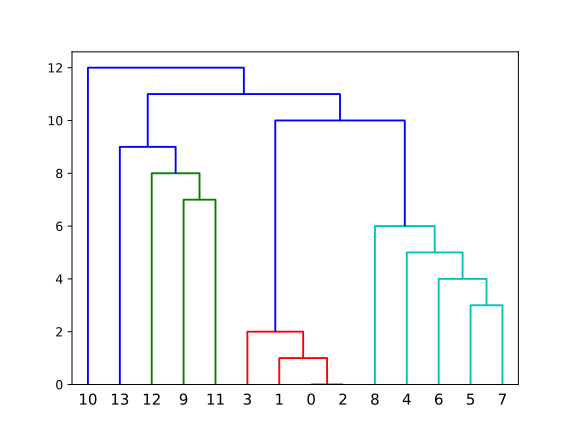
\includegraphics[width=0.49\textwidth]{img/extract_ex_dendro.png}
        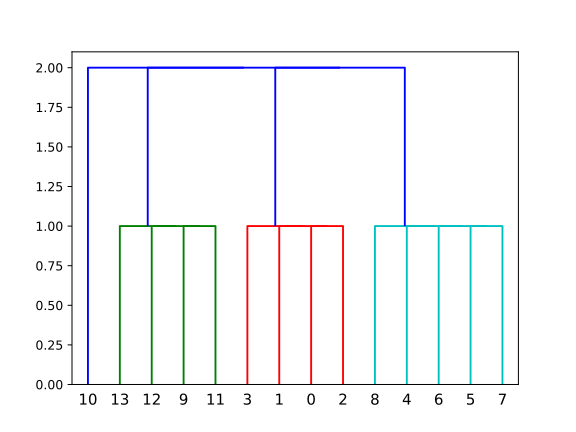
\includegraphics[width=0.49\textwidth]{img/extract_ex_taxo.png}
    \caption{The Input and output of the taxonomy extraction heuristic}
    \label{fig:my_label}
\end{figure} 
 
 \subsection{Evaluation \& Visualization}\label{\positionnumber}
 In order to evaluate the so extracted taxonomy, a way of measuring the deviation from the ground truth is needed. The Tree Edit Distance is a measure defined as the minimum cost sequence of edit operations to a tree $T$ to transform it to another tree $T'$~\cite{Tai:1979:TCP:322139.322143}. A computationally more efficient and less memory consuming implementation is APTED by Pawlik et al~\cite{pawlik2016tree}, which is used for evaluation. The visualization provides illustrations of the dendrogram, the taxonomy, the flat clusters and the resulting tree edit distance.

\section{Phase 2: Graph-aware Taxonomy Inference}\label{\positionnumber}
In the second phase the clustering algorithm is fixed to Cobweb as 
\begin{itemize}
    \item it's able to deal with all kinds of values without pre-processing, even missing values and faulty values
    \item it's hierarchical, producing not a dendrogram but rather a data driven hierarchy of variable branching factor, that is no post-processing is needed
    \item regarding Cobweb, the limiting factor is not memory, i.e. it's potentially more scalable to very large data sets
    \item it has a probabilistic (i.e. easily interpretable as fuzzy) concept description, i.e. there is no need for a fuzzy intersection or any other intermediate steps and it provides additional statistics regarding the values and their support in the data set
    \item Cobweb does not have additional parameters that need to be optimized
\end{itemize}
However note that any of the other approaches can also be used. Some of the practical problems that are discussed in the next chapter may easily be solved, so the following is a general purpose strategy for clustering in graph context, leveraging the underlying structure in the graph as well as object descriptions given by attribute value pairs.
Pre-processing and clustering is combined in this approach, as feature extraction is generally considered as a pre-processing step~\cite{han2011data}, but the feature-extraction already involves clustering. \\
The first step of the pre-processing/clustering phase \fullref{4.3.3.1} elaborates on the extraction of purely attribute value-based features and takes a rather object-oriented view on the problem of clustering in the property graph model, but is also applicable on non-graph structures. Instead of clustering nodes and edges, apply the technique to all different kinds of objects in the problem context, to obtain those features. 
The second step focuses on structural features to be extracted from the data base. The third step considers the final clustering step.


\subsection{Data Generation: The LDBC SNB Benchmark}
\fig{img/ldbc_snb.png}{ldbc}{The schema for the LDBC SNB benchmark}{0.5}
The Linked Data Benchmark Council (LDBC) consists of a group of industrial and academic organizations that research on data bases e.g. the Technische Universitaet Muenchen, Neo4J or the Vrije Universiteit Amsterdam. The LDBC social network benchmark aims at providing the following to the users:
\begin{itemize}
    \item Cover most demands that arise when managing data
    \item Modular structured, i.e. may be broken into pieces without large overhead
    \item Balanced selection of challenges
    \item Modest implementation cost
    \item Reproducibility and documentation
\end{itemize}
The synthetic data set that is generateable using the software provided by the LDBC mimics a social network that follows the schema in fig. \ref{fig:ldbc}. To ensure realism the authors modeled data link distributions as found in real world social networks like Facebook and provided attribzte values found in DBpedia. They also pay attention to regularities like homophily in the links of social networks, i.e. in a social context there tend to be more connections between people that behave similar and have similar interests. To ensure scalability of the generation process, it is implemented using the MapReduce paradigm.

\subsection{Data Loading: Neo4J Data Set Import}
Loading a data set in Neo4J requires adding it to the data base. As each data set shall reside in an own data base, each needs to be imported in an own instance of Neo4J, either using a query or an import tool. When the import has finished, all nodes and edges are traversable in Neo4J and certain statistics e.g. the node degree are available for querying from within the system. 

\subsection{Pre-Processing \& Clustering}
\subsubsection{Generalizing Node and Relationship Instances}\label{\positionnumber}
In order to discover sub-types and possible generalizations, the goal of the first step is to group all kinds of classes in an own Cobweb tree. Having an own tree for each kind is not required but reduces negative effects of ordering. There are extensions to the Cobweb framework to reduce ordering effects after insertion, that may be considered for future work. \\
In the property graph model that is one Cobweb tree for the nodes and one for the edges. What each of these trees captures are all possible node and edge sub-types present in the data set, grouped by properties and labels for nodes or relationship type for edges. Essentially the output then represents the underlying distribution of attribute value pairs. That is combining all information of the so constructed trees should be sufficient to generate a new data set that has similar objects compared to the one used for extraction, i.e. the distribution of object descriptions is partitioned and  learned. \\
In order to generalize one can set a cutoff level and replace the properties of the current node or relationship with the concept label at the chosen level. For instance when looking at road network nodes (crossings) which have no properties and edges (roads) where all roads have the same type and possibly distinct distances (e.g. 1 Km or 50 Km) the output of the procedure would optimally yield partitions based on the road length. Adding more properties like the road width would then yield sub-types like long and wide, short and tight etc. From an intuitive point of view this makes a lot of sense as humans also categorize roads by their attributes (e.g. a long and wide street is very likely a motor way, a long and medium wide street is a country road, a short and tight road is in a rather residential area, a short and wide road is probably a major city road and so on). \\
We want to infer labels, i.e. features for nodes, so why clustering and generalizing relationships? When generalizing relationships similar ones aggregate in type, so a node that has a lot of conceptually different ones may be differentiated by a node that has only relationships of one conceptual type. \\
egoDegPerType

\subsubsection{Extracting Structural Features}\label{\positionnumber}
As we focus on a label hierarchy we want to extract structural features from the nodes (compare with \fullref{2.1}: Nodes have labels, relationships have a type).
When no properties are present at all then strucutral features are the information that can be extracted. Following the approach of Henderson et al. and Neumann et al. described in \fullref{3.5} the features that are extracted are
\begin{itemize}
    \item the degree of the node
    \item the average neighbour degree
    \item the degree per relationship type of the node (also capturing the characteristic set)
    \item the average degree per relationship type of the neighbours (also capturing the average characteristic set of the neighbours)
    \item The amount of relationships that are outgoing from the ego net
    \item the amount of relationships that are incomming to the egonet
\end{itemize}
As the proposed method shall be a proof of concepts, the extracted features are neither complete nor exhaustive. Additionally weighted, directed and recursively aggregated versions of the above should also be considered.

\subsubsection{Clustering the Feature Vector}
Adding all so extracted features together produces a summary of the node that contains the following information:
\begin{itemize}
    \item Node property concept label
    \item Aggregated relationship property concepts
    \item structural features
\end{itemize}
Note that more semantic or concept-based features can be extracted, like aggregated neighbour property concepts or regarding relationships what node property types are connected by a certain edge concept. 
Applying Cobweb to those feature vector yields something similar to Henderson's role extraction~\cite{henderson2012rolx}, but with additional information: Not only the role is analyzed but also the characteristics of the object itself. What is captured as concepts in the hierarchy or taxonomy constructed by Cobweb is how a node generally looks like, that is the distribution over the properties a node has, the relation a node has and of what type the relations are. \\
Returning to the road network example this would classify the crossings by the street types and their properties, meaning that a motor way junction (a few wide long streets crossing) should end up in a different concept than a country road crossing (a few long but not too wide streets crossing). This is of course dependent on the cutoff level chosen. \\
From a theoretical point of view the proposed method is able to deal with object-oriented data, triplets like in RDF and a mixture of both models, that is the property graph model. It's able to summarize information and extract probabilistic concepts from relations, components and thereof constructed objects and graphs in a parameter-free and unsupervised manner. 


\subsection{Evaluation \& Visualization}
Again, the Tree Edit Distance and the APTED implementation is used to compare the extracted concepts to the ground truth. In this case the ground truth is the LDBC SNB schema as defined in the specification. The visualization


\section{Implementation}
\subsection{Phase 1}
% TODO quote sklearn, pyclustering, trestle
The implementation of phase 1 uses Python 3, SciKit-learn and PyClustering as basis. Overall 16 different algorithms have been tried, where only 4 of them are described in this thesis for the sake of brevity. During the implementation and experimentation the author found a bug in SciKit-learn and fixed it. As most of the algorithms require parameters a parameter optimization technique was applied namely Grid Search. In order to use the Grid Search whichs implementation is in sklearn with PyClustering, a wrapper around the algorithms of the latter was implemented. For conceptual clustering the TRESTLE algorithm from the concept formation package was used.


\subsection{Phase 2}
% TODO cite cypher
In order to implement the proposed method using Neo4J and potentially move it to a deeper level in the architecture of the data base it was implemented as a Cypher procedure that can be called from the query language. The implementation of Cobweb was done by the author from scratch as well as all feature extraction traversals of the graph, besides the node degree. For testing purposes, a annotation-based data base setup and import framework was written, provided by Manuel Hotz and refine by the author. \\
In order to boost the computational performance a multi-threaded version was implemented but yielded high contention that cancelled the concurrency gains in Cobweb. Clustering nodes and edges and extracting structual features concurrently resulted in a noticable performance gain. There is further space for optimization regarding memory access patterns, caching and storing intermediate values to avoid the computation of the same value over and over again. A more comprehensive discussion of the improvals to the method itself and the run time can be found in \fullref{6}. \\

\cleardoublepage
 \chapter{Evaluation}\label{\positionnumber}
 As briefly mentioned in \fullref{2}, different algorithms yield different clusterings as well as the same clustering with different features and parameters yields different clusterings. Thus in order to find a suitable taxonomy extraction method for the property graph model the following steps are subsequently performed:
\begin{enumerate}
    \item Algorithm Selection: Find a suitable clustering algorithm that produces a taxonomy using a minimal feature vector and different parameters to cover the space of algorithms and parameters as extensively as feasible.
    \item Feature Vector Extension: Find a suitable feature vector that also leverages the graph structure.
\end{enumerate}
In the subsequent sections, the methods and steps taken is described for each of the two steps.
 Each step has its own requirements and objectives that are addressed in the subsequent sections, but both follow the same pipeline depicted in \fullref{fig:pipeline}. \\


\section{Tag-based clustering}\label{\positionnumber}
Tag-based clustering was mainly applied in order to probe a range of different algorithms.
The selection of a fitting algorithm has three main requirements:
\begin{itemize}
    \item Memory usage: Databases need a certain amount of memory to work, so the clustering algorithm must not use all memory to cluster data. That is the memory complexity shall be as low as possible
    \item Run time: The algorithm needs to have a decent run time complexity or must provide possible optimizations to scale it to large and very large data sets (i.e.~millions of nodes, tens of millions of edges).
    \item Adaptive to nominal and numeric data: Most databases support a couple of data types, that may be summarized as either nominal (string, characters, Boolean, $\dots$) or numeric (integer, long, floats, $\dots$), i.e.~the clustering algorithm needs to be able to support both kinds of data.
    \item Noise detection and tolerance: As there are frequently missing fields in data records the clustering algorithm should be tolerant to noise and detect noisy instances.
\end{itemize}
 In order to evaluate the so extracted taxonomy, a way of measuring the deviation from the ground truth is needed. The Tree Edit Distance is a measure defined as the minimum cost sequence of edit operations to a tree $T$ to transform it to another tree $T'$~\cite{Tai:1979:TCP:322139.322143}. A computationally more efficient and less memory consuming implementation is APTED by Pawlik et al~\cite{pawlik2016tree}, which is used for evaluation. The visualization provides illustrations of the dendrogram, the taxonomy, the flat clusters and the resulting tree edit distance.

\subsection{Setup}
\subsubsection{Data}\label{\positionnumber}
Inspired by the example given in \fullref{4.1} a synthetic data set is generated, that constructs tag sets yielding a homogeneous taxonomy with a user-defined height and width when extracting the taxonomy by hand. The height is the number of levels in the hierarchy and the width is the number of children each inner node has. This allows to measure the extracted hierarchy against a simple ground truth. \\
Data sets are by nature incomplete and noisy due to measurements or human errors.
So the data generator shall also be able to introduce noise, i.e.~to add, remove or alter labels in the label set of an object in order to measure the robustness of the taxonomy extraction method. 
An example of the generated data is shown in \fullref{tab:datagen}.
\begin{table}[htp]
     \centering
     \begin{tabular}{c c} \toprule
            Node.name & Node.labels \\ \midrule
            0 & l0, l00 \\ 
            1 & l0, l01 \\ 
            2 & l0, l02 \\ 
            3 & l1, l10 \\ 
            4 & l1, l11 \\ 
            5 & l1, l12 \\
            6 & l2, l20 \\ 
            7 & l2, l21 \\ 
            8 & l2, l22 \\ \bottomrule
        \end{tabular}
    \caption{A sample of generated data for parameters height = 2, width = 3 and noise = 0 }
    \label{tab:datagen}
\end{table}{}

\noindent Synthetic data provides fine grained control over noise and a ground truth to compare against. The parameters for height and width given in \fullref{tab:synthetic_params} are used for generation, where the height defines the number of levels in the resulting hierarchy and the width describes the number of children that each non-leaf node has. For each of them $0\%$, $5\%$, $10\%$, $20\%$, $33\%$ noise is applied. This is done for each number of samples specified in the \fullref{tab:synthetic_params}.
\begin{table}[htp]
     \centering
     \begin{tabular}{|c|c|c|} \hline
            No. Samples & Width & Depth \\ \hline \hline
            243 & 3 & 5 \\ \hline
            512 & 8 & 3 \\ \hline
            1024 & 4 & 5 \\ \hline
            1331 & 11 & 3 \\ \hline
            1728 & 12 & 3 \\\hline
            2197 & 13 & 3 \\ \hline
            2401 & 7 & 4 \\ \hline
            3125 & 5 & 5 \\ \hline
            4096 & 4 & 6 \\ \hline
            6561 & 9 & 4 \\ \hline
        \end{tabular}
    \caption{The parameters used during evaluation in the synthetic data generator.}
    \label{tab:synthetic_params}
\end{table}{}

\subsubsection{Implementation}
In order to probe as many algorithms as possible and in a representative way, state of the art implementations of scikit-learn~\cite{scikit-learn} and PyClustering have been used. Overall 16 different clustering algorithms have been tried, where only 8 of them are described in this thesis for the sake of brevity. During the implementation and experimentation the author found and fixed a bug in the widely used scikit-learn package. As most of the algorithms require parameters a parameter optimization technique was applied namely random search, with the silhouette coefficient as optimization criterion. In order to use the random search --- whose implementation is using the sklearn API --- with PyClustering, a wrapper around the algorithms of the latter was implemented. For conceptual clustering the TRESTLE algorithm from the concept formation package was used, that is an extension of Cobweb that tries to rename variables and restructure data to maximize the category utility when fitting it to the root node. \\

\noindent The pipeline was then executed on a machine with two (dual slot) 64-bit AMD EPYC 7531 16 core processors, clocked at 2.4GHz with 512GiB 2666MHz DDR4 RAM, an Intel 660P NVMe SSD running 64-bit Linux 4.15 (Ubuntu). Regarding Python the Anaconda distribution, version 1.7.2 implementing Python 3.7.3 was used, along with scikit-learn 0.22 and PyClustering 0.9.2.

\subsection{Results}\label{\positionnumber}
 The run time comparison of the algorithms described in \fullref{3} is shown in \fullref{fig:rt}. 
 \begin{figure}
\centering
\begin{tikzpicture}
    \begin{axis}[
        title=Runtime Results,
        width=0.5\textwidth,
        legend pos=outer north east,
        legend style={draw=none},
        axis lines = left,
        ymax = 1000.0,
        xlabel = Samples,
        ylabel = Runtime in s,
        grid=major,
        legend entries={DBSCAN,HDBSCAN,k-Means, OPTICS, RobustSingleLinkage, SingleLinkage, Trestle, TTSAS},
        %xtick=data
    ]
        \addplot [red, mark=x] file {data/part1/runtime/synth_DBSCAN_rt.dat};
        \addplot [blue, mark=square] file {data/part1/runtime/synth_HDBSCAN_rt.dat};
        \addplot [green, mark=*] file {data/part1/runtime/synth_KMeansWrapper_rt.dat};
        \addplot [black, mark=triangle] file {data/part1/runtime/synth_OPTICS_rt.dat};
        \addplot [cyan, mark=diamond] file {data/part1/runtime/synth_RobustSingleLinkage_rt.dat};
        \addplot [teal, mark=o] file {data/part1/runtime/synth_SingleLinkage_rt.dat};
        \addplot [brown, mark=square*] file {data/part1/runtime/synth_Trestle_rt.dat};
        \addplot [magenta, mark=+] file {data/part1/runtime/synth_TTSASWrapper_rt.dat};
    \end{axis}
\end{tikzpicture}
\caption{Run time comparison of the different algorithms discussed.} \label{fig:rt}
\end{figure}

\noindent First of all some of the search spaces of the parameter optimization got limited due to performance issues (e.g. when an algorithm ran for 10 hours+ with a sample size lower than 5000). More concretely there were two such algorithms namely OPTICS and TTSAS. From an algorithmic point of view the repeated neighbourhood queries for different $\epsilon$ values impose a high linear factor, especially when choosing an epsilon value close to 1 when using Jaccard distance. Thus the maximal considered neighbourhood region was $\epsilon = 0.5$. Similarly for TTSAS, if the thresholds are too far away from each other, both too low or too high (too high means the higher threshold is greater than one and the lower close to 1), the run time degenerates to cubic and the results are rather poor. Thus the thresholds distributions were uniform between $[0.4, 0.75]$ and $[0.75, 1]$. Single Linkage has the highest run time, but sometimes intersects other algorithms, which is surprising given the fact that it has the highest computational complexity of all the methods. When investigating the implementation, it becomes clear that single linkage has the most mature and optimized implementation using Cython (that is C bindings) resulting in faster execution times for some corner cases. Robust Single Linkage performs better in most cases and one can see, that Robust Sinlge Linkage also bounds HDBSCAN as its most computationally intensive part. TTSAS and k-Means perform well for small sample sizes, but do not scale too well to larger ones. In case of TTSAS the experiment with 6561 samples resulted in a run time of approximately 3400s which is probably due to sub-optimal thresholds. OPTICS is always lower bounded by DBSCAN and upper bounded by HDBSCAN. DBSCAN is the most basic variant of the considered density-based approached, thus has to lowest run time for all larger sample sizes. Trestle performs similar to HDBSCAN and Robust Single Linkage. \\


\noindent As the resulting tree edit distance correlates with the tree size and depth (in a larger tree there are more possible edits and more possible non-matching branches when inferring a tree), there are overall 3 visualizations, showing the tree edit distance depending on the introduced noise: 
\begin{itemize}
    \item \fullref{fig:ted4096} for a 4096 samples so for a hierarchy with depth 6 and width 4
    \item \fullref{fig:ted6561} for 6561 samples that is for a hierarchy with depth 4 and width 9
    \item \fullref{fig:tednorm} shows the averaged values, i.e.~$\frac{\text{Tree Edit Distance}}{|\text{samples}|}$ as function of noise independent of depth %% Averaged
\end{itemize}

 \begin{figure}
\centering
\begin{tikzpicture}
    \begin{axis}[
        title=Qualitative Results,
        width=0.3\textwidth,
        legend pos=outer north east,
        legend style={draw=none},
        axis lines = left,
        xlabel = Noise,
        ylabel = Tree Edit Distance,
        grid=major,
        legend entries={DBSCAN,HDBSCAN,k-Means, OPTICS, RobustSingleLinkage, SingleLinkage, Trestle, TTSAS},
        %xtick=data
    ]
        \addplot [red, mark=x,samples=5] file {data/part1/ted/DBSCAN_ted_4096.dat};
        \addplot [blue, mark=square, samples=5] file {data/part1/ted/HDBSCAN_ted_4096.dat};
        \addplot [green, mark=*, samples=5] file {data/part1/ted/KMeansWrapper_ted_4096.dat};
        \addplot [black, mark=triangle, samples=5] file {data/part1/ted/OPTICS_ted_4096.dat};
        \addplot [cyan, mark=diamond, samples=5] file {data/part1/ted/RobustSingleLinkage_ted_4096.dat};
        \addplot [teal, mark=o, samples=5] file {data/part1/ted/SingleLinkage_ted_4096.dat};
        \addplot [brown, mark=square*, samples=5] file {data/part1/ted/Trestle_ted_4096.dat};
        \addplot [magenta, mark=+, samples=5] file {data/part1/ted/TTSASWrapper_ted_4096.dat};
    \end{axis}
\end{tikzpicture}
\caption{Tree Edit Distance per noise level for 4096 samples} \label{fig:ted4096}
\end{figure}

\begin{figure}
\centering
\begin{tikzpicture}
    \begin{axis}[
        title=Qualitative Results,
        width=0.3\textwidth,
        legend pos=outer north east,
        legend style={draw=none},
        axis lines = left,
        xlabel = Noise,
        ylabel = Tree Edit Distance,
        grid=major,
        legend entries={DBSCAN,HDBSCAN,k-Means, OPTICS, RobustSingleLinkage, SingleLinkage, Trestle, TTSAS},
        %xtick=data
    ]
        \addplot [red, mark=x, samples=5] file {data/part1/ted/DBSCAN_ted_6561.dat};
        \addplot [blue, mark=square,  samples=5] file {data/part1/ted/HDBSCAN_ted_6561.dat};
        \addplot [green, mark=*,  samples=5] file {data/part1/ted/KMeansWrapper_ted_6561.dat};
        \addplot [black, mark=triangle,  samples=5] file {data/part1/ted/OPTICS_ted_6561.dat};
        \addplot [cyan, mark=diamond,  samples=5] file {data/part1/ted/RobustSingleLinkage_ted_6561.dat};
        \addplot [teal, mark=o,  samples=5] file {data/part1/ted/SingleLinkage_ted_6561.dat};
        \addplot [brown, mark=square*,  samples=5] file {data/part1/ted/Trestle_ted_6561.dat};
        \addplot [magenta, mark=+,  samples=5] file {data/part1/ted/TTSASWrapper_ted_6561.dat};
    \end{axis}
\end{tikzpicture}
\caption{Tree Edit Distance per noise level for 6561 samples} \label{fig:ted6561}
\end{figure}

 \begin{figure}
\centering
\begin{tikzpicture}
    \begin{axis}[
        title=Qualitative Results,
        width=0.3\textwidth,
        legend pos=outer north east,
        legend style={draw=none},
        axis lines = left,
        xlabel = Noise,
        ylabel = $\frac{\text{Tree Edit Distance}}{|\text{samples}|}$,
        grid=major,
        legend entries={DBSCAN,HDBSCAN,k-Means, OPTICS, RobustSingleLinkage, SingleLinkage, Trestle, TTSAS},
        %xtick=data
    ]
        \addplot [red, mark=x,samples=5] file {data/part1/ted/DBSCAN_ted_norm.dat};
        \addplot [blue, mark=square, samples=5] file {data/part1/ted/HDBSCAN_ted_norm.dat};
        \addplot [green, mark=*, samples=5] file {data/part1/ted/KMeansWrapper_ted_norm.dat};
        \addplot [black, mark=triangle, samples=5] file {data/part1/ted/OPTICS_ted_norm.dat};
        \addplot [cyan, mark=diamond, samples=5] file {data/part1/ted/RobustSingleLinkage_ted_norm.dat};
        \addplot [teal, mark=o, samples=5] file {data/part1/ted/SingleLinkage_ted_norm.dat};
        \addplot [brown, mark=square*, samples=5] file {data/part1/ted/Trestle_ted_norm.dat};
        \addplot [magenta, mark=+, samples=5] file {data/part1/ted/TTSASWrapper_ted_norm.dat};
    \end{axis}
\end{tikzpicture}
\caption{Tree Edit Distance per noise level divided by sample size} \label{fig:tednorm}
\end{figure}

\noindent One can clearly see, that single linkage is by design not able to group objects that have equivalent attributes in one cluster in a single step, but rather in subsequent steps, resulting in a very high tree edit distance. Robust Single Linkage provides great improvements over classic Single Linkage, as it allows merging multiple objects at once and only merges multiple objects when appropriate. The density-based methods are quite similar when it comes to the tree edit distance, i.e.~very robust to noise, but only in rare cases exact. k-Means is always worse than the density-based approach in terms of the tree edit distance, like TTSAS even tough TTSAS is able to reach similar TED scores as the density-based approach. Trestle is the only algorithms whose performance decreases with the introduced noise and the only algorithm that improves with the height of the ground truth hierarchy. This is especially noticable when comparing \fullref{fig:ted4096} with \fullref{fig:ted6561}, where the point of intersection between Trestle and the density-based approaches is at a higher noise level compared due to 2 more steps in the hierarchy as compared to the latter figure where this intersections happens almost at 0 nosie. This is due to the fact that it is the only algorithm able to change the depth of the inferred hierarchy through out the whole processing step. 

\subsection{Discussion}\label{\positionnumber}
The results with respect to time only focus on the clustering time itself. When looking at multi-phase approaches and robust single linkage, we have to keep in mind that those algorithms have parameters that need to be inferred to obtain meaningful results. Depending on the parameter space and the inference method this may take a dominant amount of time as each iteration in the inference process must use at least some representative sample of the data and execute the full algorithm on that. For example a randomized search samples parameters from used-defined distributions a pre-defined number of times and executes the algorithm on the whole data set to evaluate the results with respect to a user defined measure. This may result in factors of more than 100 for medium and large parameter spaces with non-trivial restrictions of the parameters. However note, that also the inference of parameters is of course highly dependent on an appropriate choice of the parameter distribution or restricted space (depending on inference methodology). That is the presented run times are not guaranteed to be globally optimal, but rather the local optimum found by the randomized search. \\
Additionally the vectorization of categorical attributes that is necessary for all algorithms besides Trestle --- or more generally conceptual clustering approaches --- uses additional space, that is equivalent to the number of distinct values of all attributes, what may grow relatively large. Although this amount of memory may be freed when the distance matrix is computed, one needs the memory for both the objects including vectorized attributes and the distance matrix. For large data sets this is infeasible and provides little possibilities for optimization. One would be explicit swapping when iterating over the elements during distance computation, so that at any time only a part of the matrix would be in main memory as well as only a couple of objects at a time. This may be achieved using a database and an implementation that does I/O similarly to the two-way merge sort algorithm. \\
Another issue is that of noisy data sets. When there is too much noise, the intersection of the attributes in a cluster may be empty, resulting in unusable object descriptions and non-sense hierarchies that get extracted. Additionally there is the need to flatten the dendrogram that is produced during Single Linkage Clustering, which can only unify subsequent merges but not restructure the merges in general. \\
Some of the so far evaluated approaches may be applied to the graph-aware pipeline, when integrating them more closely with the memory optimization facilities of a database in mind and further refinements, like introducing a fuzzy intersection to describe cluster representatives in the multi-phase approach.
        

\section{Graph-aware clustering of Nodes}\label{\positionnumber}
Conceptual clustering provides a lot of useful traits for this application: 
\begin{itemize}
    \item Parameter-free: As Cobweb does not need additional parameters, there is no need to tune those i.e.~the algorithm fits to the data by its' own means in theory.
    \item Memory: It is incremental and thus uses in the most inefficient implementation $\mathcal{O}(n)$ memory. Does not require vectorization or similar things.
    \item Computation: Generally Conceptual clustering is able to integrate a node in logarithmic time with respect to the number of already incorporated instances, but also requires  $B + 4 \cdot 3B \cdot A \cdot 2V$ floating point computations, which may grow very large, depending on the number of attributes and values. Finding an objective function that is rank-preserving and uses less computations, reducing the number of occasions where the objective function is computed and a way to only select the most discriminating attributes provides means for optimization of the computational complexity.
    \item Probabilistic concept descriptions: The problem of an empty intersection is overcome by using probabilistic concept descriptions, that may also provide further helpful information in query optimization.
    \item Hierarchical: Producing not a dendrogram but rather a data driven hierarchy of variable branching factor, that is no post-processing is needed.
    \item Existing extension to mixed data without additional memory or computational complexity. \\ 
    In contrast to what McKusick et al. reports (``[...] summing together terms from both forms of the equation works well in domains with mixed data.``)~\cite{mckusick1990cobweb}, mixed data processing was dominated by numeric values, thus a constant bias was added to the denominator of the equation for continuous values in \fullref{3.4.2}.
\end{itemize}
For this reason Cobweb is used for the evaluation of the graph-aware pipeline. Density-based algorithms in combination with robust single linkage may provide superior robustness and faster run times, but also require further adaptions which introduce additional degrees of freedom. As we want to experiment with different feature vectors this is undesirable here and we stick with the maybe sub-optimal but more convenient cobweb algorithm. \\

\subsection{Setup}\label{\positionnumber}
\subsubsection{Data}
\fig{img/ldbc_snb.png}{ldbc}{The schema for the LDBC SNB benchmark}{0.7}
The Linked Data Benchmark Council (LDBC) consists of a group of industrial and academic organizations that research on databases e.g. the Technische Universitaet Muenchen, Neo4j or the Vrije Universiteit Amsterdam. The LDBC social network benchmark aims at fulfilling the following requirements:
\begin{itemize}
    \item Cover most demands that arise when managing data
    \item Modular structured, i.e.~may be broken into pieces without large overhead
    \item Balanced selection of challenges
    \item Modest implementation cost
    \item Reproducibility and documentation
\end{itemize}
The synthetic data set that is generateable using the software provided by the LDBC mimics a social network that follows the schema in \fullref{fig:ldbc}. To ensure realism the authors modeled data link distributions as found in real world social networks like Facebook and provided attribute values found in DBpedia. They also pay attention to regularities like homophily in the links of social networks, i.e.~in a social context there tend to be more connections between people that behave similar and have similar interests. To ensure scaling ability of the generation process, it is implemented using the MapReduce paradigm.
\noindent The LDBC SNB dataset is used to probe the pipeline as some sort of ground truth is available, even though this ground truth only considers node labels in the sense of a label in Neo4j rather than similar instances. The cardinalities of instances in the database is a dominant factor for deriving such a hierarchy. For example consider a sample size of 10000. If 9950 of 10000 samples are instances with the node label message, the output of a taxonomy will mainly provide characteristics of nodes with those labels while nodes with other labels are a minority and may even be classified as noise.
  Additionally the yelp data set is used as an example for a not graph but rather ``object-oriented`` or property-oriented data set. 
  One experiment uses the New York Road Net data set provided by the 9th DIMACS shortest path challenge to demonstrate the pipeline on a less complex and spatially graph-oriented data set~\cite{9thDIMACSImplementationChallengeShortestPaths-2010-06-14}.
  
\subsubsection{Pre-Processing}
Cobweb is able to deal with character strings by design, while all other clustering algorithms introduced in \fullref{3} require dictionary vectorization as pre-processing step.
  \noindent A number of different combinations of the following features has been used:
\begin{itemize}
    \item the labels of the nodes $V, L, f_l$ 
    \item the properties of the nodes
    \item per node structural features of the underlying graph that is the node degree, the average neighbour degree, the number of nodes incoming to the ego net and the number of nodes outgoing from the ego net
    \item the characteristic set of a node, that is the set of all relation types associated with this node 
\end{itemize}
The node labels have always been used. For the latter three features, all variations (i.e.~the labels plus one element of the power set) have been tried. \\
  
  \subsubsection{Implementation}
  In order to integrate the proposed method with Neo4j and potentially move it to a deeper level in the architecture of the database it was implemented as a Cypher procedure so that it complies with the internal API of Neo4j and can be called from the query language Cypher. The implementation of Cobweb was done by the author from scratch as well as all feature extraction traversals of the graph, besides the node degree. \\
The implementation of Cobweb uses the adjusted category utility from ~\cite{mckusick1990cobweb} and an unbiased and numerically stable algorithm for computing mean and variance, namely Chan's Algorithm~\cite{chansAlgo} as proposed by MacLellan et al~\cite{maclellan2016trestle}.
For testing purposes, an annotation-based database setup and import framework was written, provided by Manuel Hotz and refined by the author. \\
In order to boost the computational performance a multi-threaded version was implemented but yielded high contention that cancelled the concurrency gains in Cobweb. There is further space for optimization regarding memory access patterns, caching and storing intermediate values to avoid the computation of the same value over and over again. \\

The pipeline was again executed on a machine with two (dual slot) 64-bit AMD EPYC 7531 16 core processors, clocked at 2.4GHz with 512GiB 2666MHz DDR4 RAM, an Intel 660P NVMe SSD running 64-bit Linux 4.15 (Ubuntu). Regarding Java the OpenJDK distribution, version 11.0.4 was used, along with Neo4j 3.5.3.

\subsection{Results}\label{\positionnumber}
In \fullref{fig:ldbctree} the ground truth label hierarchy is shown.
\begin{figure}
    \centering
    \begin{figure*}[t]
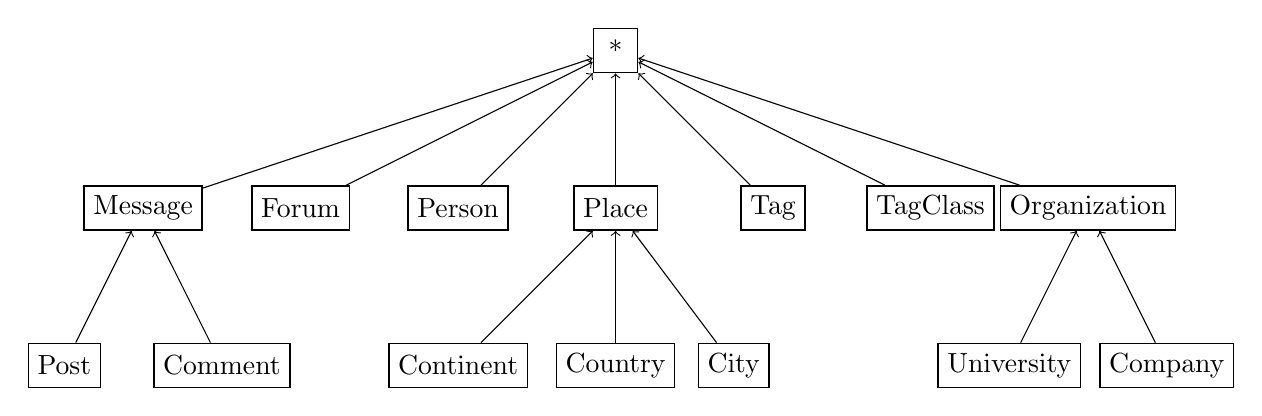
\begin{tikzpicture}
\node[draw=black,minimum size = 16pt,line width = 0.5pt,] at (0, 0)  		(ROOT)	{*};
\node[draw=black,minimum size = 16pt,line width = 0.5pt,] at (-6, -2) 	(N1) 	{Message};
\node[draw=black,minimum size = 16pt,line width = 0.5pt,] at (-4, -2) 	(N2)	{Forum};
\node[draw=black,minimum size = 16pt,line width = 0.5pt,] at (-2, -2) 	(N3) 	{Person};
\node[draw=black,minimum size = 16pt,line width = 0.5pt,] at (0, -2)  	(N4) 	{Place};
\node[draw=black,minimum size = 16pt,line width = 0.5pt,] at (2, -2)  	(N5) 	{Tag};
\node[draw=black,minimum size = 16pt,line width = 0.5pt,] at (4, -2)  	(N6) 	{TagClass};
\node[draw=black,minimum size = 16pt,line width = 0.5pt,] at (6, -2)  	(N7)	{Organization};
\node[draw=black,minimum size = 16pt,line width = 0.5pt,] at (-7, -4) 	(N11) 	{Post};
\node[draw=black,minimum size = 16pt,line width = 0.5pt,] at (-5, -4) 	(N12) 	{Comment};
\node[draw=black,minimum size = 16pt,line width = 0.5pt,] at (-2, -4)  	(N41) 	{Continent};
\node[draw=black,minimum size = 16pt,line width = 0.5pt,] at (0, -4)  	(N42) 	{Country};
\node[draw=black,minimum size = 16pt,line width = 0.5pt,] at (1.5, -4)  	(N43) 	{City};
\node[draw=black,minimum size = 16pt,line width = 0.5pt,] at (5, -4)  	(N71)	{University};
\node[draw=black,minimum size = 16pt,line width = 0.5pt,] at (7, -4)  	(N72)	{Company};
\draw[<-] (ROOT) -- (N1);
\draw[<-] (ROOT) -- (N2);
\draw[<-] (ROOT) -- (N3);
\draw[<-] (ROOT) -- (N4);
\draw[<-] (ROOT) -- (N5);
\draw[<-] (ROOT) -- (N6);
\draw[<-] (ROOT) -- (N7);
\draw[<-] (N1) -- (N11);
\draw[<-] (N1) -- (N12);
\draw[<-] (N4) -- (N41);
\draw[<-] (N4) -- (N42);
\draw[<-] (N4) -- (N43);
\draw[<-] (N7) -- (N71);
\draw[<-] (N7) -- (N72);
\end{tikzpicture}
\caption{Label hierarchy for the SNB database.}
\end{figure*} 

    \caption{Ground truth label hierarchy for the LDBC SNB data set}
    \label{fig:ldbctree}
\end{figure}{}
The trees visualized in the following section are the label hierarchies that were inferred with generated abstract labels. That means the labels in the trees shown as result have no semantic meaning and are solely there to reference the table describing the same concept as the node. Also the root of the tree is always called ``Root`` as it always contains an aggregation of all values present in the feature vector for all incorporated nodes. The tables for all concepts shown in the trees can be found in the appendix. An exemplar table is shown in \fullref{lldbccnl0}
As the trees get relatively large due to saving each instance as an extra node, the results are cut at the second level of the tree which is mostly sub-optimal. This is a similar problem as the one of single linkage, that is further addressed in extensions of the Cobweb algorithm e.g. in \cite{classit, thompson1989incremental} and others.
We shall visually inspect differences, as due to the above mentioned difficulties, the tree edit distance may be closer to the ground truth even tough the learned concepts aren't. 
Also some values in the concept description tables are not visualized, as the tables get very large (more than 100 rows, some values wider than what fits on A4 paper). 
Many of the trees contain the desired concepts, but at levels that are not always the same, i.e.~there is no level in the tree that contains optimal concepts for all branches. 
For instance as the ratio of persons to messages is very low, the desired concept of persons may be at a very low level and the desired concept for messages is at a rather high level in the tree. 
That is concepts with high support are at a high level in the tree, while concepts with low support are at lower levels. For all the data sets a sample size of 2000 nodes and all relationships connecting to those nodes was used. \\

\paragraph{Labels Only}
When only taking the node labels into account on the LDBC SNB data set, the algorithm splits at the first level all Comments (which are also messages) and then all posts at the next level. This is also due to the cardinality of the label sets. The fact that both l0 and l10 conatin the label message is probably due to order effects described by Fisher in more detail~\cite{Fisher1987}. All other labels are present at such low total probabilities, that the split that separates those eventually is at a deeper level in the tree. The tree is shown in \fullref{fig:lldbctree} and an example for a concept description table can be found in \fullref{l0ex}. \\

\begin{figure}[htp]
    \centering
    \begin{forest}
[Root
	[l0 
		[l00 
]		[l01 
]]	[l1 
		[l10 
]		[l11 
]]]
\end{forest} \\
    \caption{Inferred Label Hierarchy with labels only}
    \label{fig:lldbctree}
\end{figure}{}
\begin{table}[H] 
  \centering 
 \begin{longtable}{|c|c|c|c|c|} \hline 
Attribute & ValueType & Value & Probability & Occurences \\ \hline 
\multirow{2}{*}{Labels} & Nominal & Message & $1.0000$ & $1289$ \\ \cline{2-5} 
 & Nominal & Comment & $1.0000$ & $1289$ \\ \hline 
 \captionsetup{position=top}
 \caption{Example concept description for node l0: P(node) = 0.6445, Count = 1289}\label{l0ex}
\end{longtable}
 \end{table} 

If the label distribution only consists of one equally probable label for all nodes there is no valuable information that can be used to cluster the data instances, thus the tree is made up of a single root node and no information is gained. An example here fore is the yelp data set with properties to store all information when it is clustered using only the label sets. That is for all nodes ``Business`` so there is only one concept containing all nodes. \\
 
 \paragraph{Labels and Node Properties}
\begin{figure}[htp]
    \centering
    \begin{forest}
[Root
	[l0 
		[l00 
]		[l01 
]]	[l1 
		[l10 
]		[l11 
]]]
\end{forest}
    \caption{Inferred Label Hierarchy for the LDBC SNB data set with labels and properties as the feature vector}
    \label{fig:lpldbctree}
\end{figure}{}
The first three levels of the generated tree is shown in \fullref{fig:lpldbctree}. When using the properties additionally to the set of labels, a sub-tree is appended at l0 splitting nodes that have labels message and comment further into messages of created with different browsers. The sub-tree starting at l1 is very similar to the one with only labels: It splits into nodes having the labels message and post and those having anything else but in contrast to before still contains nodes having the labels message and post. The unclean split is due to the extra noise introduced with the presence of the properties. As there are a lot of properties, the predictiveness of some properties (e.g. the id, what browser was used, the creation date) weakens the effect of the label predictiveness and thus introduces additional noise. \\

\begin{figure}[htp]
    \centering
    \begin{forest}
[Root
]
\end{forest}
    \caption{Inferred Label Hierarchy for the property-oriented Yelp data set with labels and properties as the feature vector}
    \label{fig:lplyelpootree}
\end{figure}{}
In the previous paragraph we noticed, that a data set with only one equi-probable label for all nodes contains no information. If a data set has node properties, adding those to the feature vector enables the use of clustering methods to extract concepts. The first three levels of the generated tree is shown in \fullref{fig:lplyelpootree}. Depending on how predictive the properties are and in how many directions they are, the resulting hierarchy may be clean but is mostly rather messy: For instance the property-based Yelp data set contains attributes describing spatial features (the exact location including latitude, longitude, address, state, $\dots$), time based features (the opening hours), numeric and nominal ones (user-defined categories, price ranges, an average review score and a review count for example). Optimizing for those in common yields a mixture of the above which introduces a lot of noise. Some semantically close instances are in different concept classes as their spatial position differs completely, while some spatially and semantically close instances are in distinct groups due to different tags assigned (covering traits like WiFi, Parking, GoodForChildren). Extensions of the algorithm to deal with Spatial and Date-based values, to find correlations in the attribute-value distribution and to evaluate only the most salient and discriminative values or weighting, cleaning and projection of properties before clustering may provide further refinements to improve the result using properties in the feature vectors. \\

Considering a road network data set, with no node labels and no properties, there is no information to cluster the nodes with, that is this feature vector yields no information for such data sets. \\

\paragraph{Labels and Characteristic Sets}
\begin{figure}[htp]
    \centering
    \begin{forest}
[Root
	[l0 
		[l00 
]		[l01 
]]	[l1 
		[l10 
]		[l11 
]]]
\end{forest} \\
    \caption{Inferred Label Hierarchy for the SNB data set with labels and the characteristic set as the feature vector}
    \label{fig:lcldbctree}
\end{figure}{}
Taking the characteristic set into account results in more information than with labels only but less noise than with the properties for most cases. Applied to the LDBC SNB data set, the concepts are similar to the ones created with labels only with some additions: l0 is again the concept that contains nodes with labels message and comment, but additionally separates between nodes that have relationships to tags, nodes that do rather not and a class where approximately two thirds of the nodes have tags. The latter one is probably created erroneously due to ordering effects. In the sub-tree of l1 again nodes with labels Message and Post are split from the rest of the nodes. There are actually two sub-concepts for nodes with labels Message and Post: One where there are mostly tagged answer posts, and one where the posts are not in reply to something and barely have tags. The first three levels of the generated tree is shown in \fullref{fig:lcldbctree}. \\

Again if we have no relationships as in the property-oriented yelp data set we gain no information by adding the characteristic set (as it is an empty set). Another case where no relevant information is gained is the case of a road network: Every node has edges with the relationship type ``ROAD``. That is all characteristic sets are exactly the same containing one element --- namely ``ROAD``. \\

\paragraph{Labels and Structural Features}
\begin{figure}[htp]
    \centering
    \begin{forest}
[Root
	[l0 
		[l00 
]		[l01 
]]	[l1 
		[l10 
]		[l11 
]]]
\end{forest} \\
    \caption{Inferred Label Hierarchy for the SNB data set with labels and structural features as the feature vector}
    \label{fig:lsldbctree}
\end{figure}{}
Here the nodes are structured as with just the labels, but additionally in the sub-tree l0 there is a distinction between lower mean node degree, lower number of outgoing edges, higher average neighbour degree and higher mean node degree, higher number of outgoing edges, lower average neighbour degree. On the sub-tree of l1 there is again the nodes having the labels message and post and those having anything else split. This time the split provides additional relevant information: nodes with labels ``Message`` and ``Post`` have mostly a low degree and a lower number of edges outgoing from the ego net but a high number of edges incoming to the ego net and a high average neighbour degree, whereas nodes with other labels have on average a higher degree, more outgoing than incoming edges to the ego net and a lower average neighbour degree. The first three levels of the generated tree is shown in \fullref{fig:lsldbctree}. Note however, that more complex structural features can be extracted in order to extract more complex meaning from the data and that a different bias term as mentioned in the first paragraph of \fullref{5.2} may change the result significantly. That is if numeric values dominate the result, the influence that the labels (nominal values) have decreases in comparison to the structural features which are numeric. This also applies for properties (mixed) and the characteristic set (nominal). \\

\begin{figure}[htp]
    \centering
    \begin{forest}
[Root
	[l0 
		[l00 
]		[l01 
]]	[l1 
		[l11 
]]	[l2 
		[l20 
]		[l21 
]		[l22 
]		[l23 
]		[l24 
]]]
\end{forest} \\
    \caption{Inferred Label Hierarchy for the New York road network data set with labels and structural features as the feature vector}
    \label{fig:lsroadnetnytree}
\end{figure}{}
For the property oriented yelp data set we have again no meaningful information gain as it does not contain any relationships. \\

For the road network example the situation looks a bit different now: Crossings connecting many streets and those who only connect two streets are separated as well as streets in more or less dense networks. The sub-tree l0 contains all crossings having exactly 3 roads that are connected. It further sub-divides into crossings whose ego nets have between 17 (l03) and 23 (l01) incoming and outgoing roads. Sub-tree l1 contains all crossings that connect exactly 1 road (dead ends). Last but not least sub-tree l3 contains crossings connecting either 2 or 4 roads with 15 and 31 incoming and outgoing roads respectively. The first three levels of the generated tree is shown in \fullref{fig:lsroadnetnytree}.


\paragraph{Labels and mixtures of the other features}
\begin{figure}[htp]
    \centering
    \begin{forest}
[Root
	[l0 
		[l00 
]		[l01 
]]	[l1 
		[l10 
]		[l11 
]]]
\end{forest} \\
    \caption{Inferred Label Hierarchy for the SNB data set with labels, structural features and the characteristic set as feature vector}
    \label{fig:lscldbctree}
\end{figure}{}
When taking labels, structural features and the characteristic set as the feature vector the resulting hierarchy is the same, if only the structure of the hierarchy is considered. The first three levels of the generated tree is shown in \fullref{fig:lscldbctree}. Semantically at the sub-tree l1 nodes with the labels Message and comment are split as for most of the example hierarchies before. The split happening after l1 separates nodes with a degree of exactly 3 (std is 0.027) from higher degree nodes with a mean degree of 9. This indicates the number of tags of the comment: The higher the degree, the more tags are attached, which is also visible from significant differences in the probabilities of the characteristic set containing the HAS\_TAG relationship ($99.5\%$ for the higher degree nodes versus $0.35\%$ for the lower degree nodes). The sub-tree l0 separates again the rest of the nodes and the children sub-divide into nodes with labels Message and Post (l01, l02) and the rest (l00). The concepts l01 and l02 separate posts with a high degree and a low degree indicating more or less tags and replies as with comments. This time the probabilities are $3,8\%$, $0.21\%$, $0\%$ versus $17\%$, $89.7\%$, $85.2\%$ for likes, tags and replies respectively. \\


\begin{figure}[htp]
    \centering
    \begin{forest}
[Root
	[l0 
		[l00 
]		[l01 
]]	[l1 
		[l10 
]		[l11 
]]]
\end{forest} \\
    \caption{Inferred Label Hierarchy for the SNB data set with labels, node properties, structural features and the characteristic set as feature vector}
    \label{fig:lpscldbctree}
\end{figure}{}
Taking the properties additionally into account introduces more noise, that is more features of for which the information gain is unknown and might be negative (that is adding the information to the feature vector actually interferes with the algorithm's ability to extract the relevant concepts with the correct attribute value distribution from the underlying data distribution). The first three levels of the generated tree is shown in \fullref{fig:lpscldbctree}. Here l0 splits again between nodes with labels message comment but in the subsequent step the predictiveness of using a certain browser is maximized which is a characteristic of the data which does not carry any further information about structure and distribution of the data. In the other sub-tree again nodes with the labels message and post are split from the nodes containing all other labels. \\


\subsection{Discussion}\label{\positionnumber}
 None of the generated concepts or label hierarchies do match fully to the ground truth, but this is also not what is desired. Desired is to extract meaningful and representative concept classes that can be used to derive labels. For example the LDBC data set contains about $95\%$ nodes with the label ``Message`` and only a very small amount of nodes with the label ``Person``. Therefore it is representative to split at the first steps into ``Message and non-Message``-labled nodes as this is the major difference between the largest group of nodes in this data set and all the others. \\
 The results clearly indicate that there is no single feature vector which can be used to extract meaningful concepts from all data sets. For data sets not leveraging graph structures, the characteristic set and structural features contain no information like in the non-transformed yelp data set. For those which do not have properties attached to the data set, taking the properties into account yields no information. Road network data like the New York road net data set contain often no labels, that is taking the labels into account in the feature vector adds no information. \\
 On the other hand, adding the properties to the feature vector may introduce additional noise and actually disturb the derivation of meaningful concepts that represent the underlying distribution. \\
 Constructing the feature vector adaptively seems to be the only option resulting in a minimal and complete source of information on the data set. That is if there are no relations but properties, only the properties and eventually the labels when meaningful shall be used. On the other hand for data sets not containing properties, useful labels and more than one relationship type, structural features are the only usable feature that should be used and so on. \\
 Also extensions to the algorithms to make the procedure detect significant correlations, deal with temporal and spatial data types (and possibly others requiring special semantics to yield useful aggregations not considered here) and the ability to only use those attributes with the highest information gain. In general it seems that both a Bayesian and an information theoretic extension of the conceptual clustering framework may counter some of the problems. Applied to the other clustering algorithms such extensions would require additional pre-processing, for instance a sampling procedure to estimate correlations and to calculate the information gain for certain attributes or groups of correlated attributes. \\
 As the distributions that shall be learned are only constrained to model numeric values as Gaussians, there is no upper bound for the sample complexity, due to the no free lunch theorem. Further when loosening the Gaussian prior which has no concrete theoretical justification the space of possible distributions is unrestricted. 

\cleardoublepage
\chapter{Conclusion}\label{\positionnumber}
\section{Summary}\label{\positionnumber}
In this thesis, a pipeline was designed in order to conduct a survey, comparing hierarchical agglomerative, density-based, partition-based and conceptual state-of-the-art clustering. More practically relevant problems with those approaches include parameter inference, space complexity and empty cluster descriptions (that is the set of all common attributes of the instances in the cluster) for noisy domains. Those could be overcome by introducing a more sophisticated parameter inference mechanism as randomized search e.g. stochastic variational inference~\cite{hoffman2013stochastic}, by implementing the computation of the distance matrix and the algorithms using it in a fashion similar to the two-way merge sort algorithm, i.e.~only using a few buffer pages keeping in ram only what is necessary for a batch of iterations and by introducing a probabilistic concept description using a fuzzy intersections for determining the cluster description. A model-based hierarchical framework namely conceptual clustering provided superior abilities regarding some characteristics, especially that the algorithm is to some degree able to deal with mixed data, has linear space complexity, is incremental and produces hierarchies by design instead of the multi-phase approach requiring additional post-processing as for the other algorithm classes. \\
This approach was used in the second part, where a graph-aware version of the previous pipeline was introduced that leverages graph-based features of the graph. Different feature vectors were evaluated, concluding that finding the features extracted have to be chosen adaptively. For example it is desirable to look at the labels and structural features only in case if there are no properties and all relationships have the same type. In the case when there are no relationships one might want to consider the properties of the node and the label as feature vector (i.e.~no structural features as they contain no information) and so on.

\section{Future Work}\label{\positionnumber}
Generally there are three categories of future work 
\begin{enumerate}
    \item Incorporate extensions to the conceptual clustering framework
    \item Find better feature vectors and ways to construct them adaptively
    \item Apply conceptual clustering or multi-phase clustering with adaptive feature vectors to other domains
\end{enumerate}{}
There are a lot of extensions to the conceptual clustering framework. Cheeseman~\cite{cheeseman1988autoclass} integrates the Bayesian interpretation more concretely into the method. Gennari~\cite{classit} reduces the number of nodes in the tree by storing pointers to the data instances instead of nodes and probabilistic concepts in the tree such that the leaves are rather the elements of a concept class than concepts themselves. Thompson et al.~\cite{thompson1991concept} takes structured domains into account and introduces internal links in the hierarchy. That is if an object from a different class is contained in the description, it may be linked and treated as entity in the hierarchy (that is a sub-concept is also part of the super-concept). The mathematical field of formal concept analysis provides a concise mathematical foundation for the framework, which Godin et al.~\cite{doi:10.1111/j.1467-8640.1995.tb00031.x} synthesised into the construction of the concepts using Gallois lattices. Xie et al.~\cite{xie2002concept} suggests the usage of the of concept lattices for classification which is similar to what Godin et al.~\cite{doi:10.1111/j.1467-8640.1995.tb00031.x} proposes. Devaney et al.~\cite{devaney1997efficient} provide an extension that focuses on the efficient selection of features. Fisher~\cite{fisher1996iterative} provides a series of improvements, that may be applied to select only features that assist the optimization process to avoid noisy concept descriptions and methods to refine the tree after an instance or all instances have been incorporated like restructuring the hierarchy or cleaning some concept descriptions. Many other improvements can be thought of like the detection of correlated features after incorporating new instances. Even tough conceptual clustering has not received much attention since the 90s it remains a field of research. \\

Finding better feature vectors includes not only the invention of better features but also the selection of the significant features and pruning of unnecessary or grouping of highly correlated features. Depending on the application use case, the adaption strategy may be far from trivial. When the features are not human readable but generated as an intermediate or internal representation as the filters that are learned during the training of a neural net, the selection of features not only from the top level but through out the network with keeping at the same time a modest number of features is an example for a non-trivial adaption procedure. \\
In the database environment, many products already contain a profile that is used for cardinality optimization which can give concrete guidelines for the features to use or not to use. \\

Cardinality estimation for query optimization has been an ongoing research topic since the invention of databases. Many different methods have been invented and applied, most of which can be divided in 2 general approaches:
\begin{itemize}
    \item Database Profile: Keep statistics about the value distributions to estimate cardinality (e.g. using general statistics about the relations, histograms, results of previous queries, $\dots$)
    \item  Sampling techniques: Execute the query with a sample of the considered relationships to
estimate cardinalities
\end{itemize}
The first approach assumes uniformity and independence assumptions when using general statistics and tries to mitigate inaccuracies by those assumptions with histograms, which accuracy depends on the chosen bucket size and which are not able to capture correlations between different attributes. Those two approaches have also been adapted to graph-based data models. 
Neumann et al. propose characteristic sets, that is the set containing all relationship types, predicates, labels or however they are called in the implementation to estimate cardinalities~\cite{neumann2011characteristic}. \\
Neo4j, the ``leading`` graph database according to it’s homepage, uses a database profile with the following statistics according to the operations manual~\cite{neo4jstatistics}:
\begin{enumerate}
    \item The number of nodes having a certain label.
    \item The number of relationships by type.
    \item  The number of relationships by type, ending or starting from a node with a specific label.
    \item Selectivity per index.
\end{enumerate}
Thus they make use of the uniformity and independence assumption and rely on indices to
provide information about property value information per label~\cite{neo4jIndex}. Further the Query Planer of Neo4j can only use one index at a time and picks a sub-optimal index sometimes~\cite{neo4jBadindex}.
Those and other weaknesses in cardinality estimation may be overcome by explicitly storing taxonomies of the data implicated in the database. Taxonomies capture differences in value distributions for similar data instances and assign those to categories which may then be used not only for cardinality estimation but also for data exploration, profiling and analysis. A feature vector that is adapted according to the already existing database profile may greatly improve the results, capturing concrete attribute-value distributions for different compositions and correlations. As Cobweb is incremental this may be implemented as a dynamic (update-able) index which is then used by the query optimizer during cardinality estimation. \\
Another interesting application is that of using taxonomies of sub-graphs as self-organizing associative index, that segments the physical storage of the data base to optimize query times in a molecule database~\cite{levinson1984self}. \\

\noindent Other use cases include cognitive architectures~\cite{langley1990integrated} and the modelling of human learning behaviour~\cite{maclellan2016trestle}. 



\cleardoublepage
\chapter{Appendix}

\section{Estimation Results}
\label{app:test-results}

The following Table \ref{table:test-results} lists the actual and estimated result
cardinality of our ("Cascades") and Neo4j's ("Neo4j") estimation model for all
queries of our SNB query
catalog (cf. Tables  \ref{table:query-catalog-1}, \ref{table:query-catalog-2} and
\ref{table:query-catalog-3}).

\begin{longtable}{llll}
\label{table:test-results} \\
\toprule
\midrule
Query Id & Result cardinality & Optimizer & Estimated cardinality \\
\midrule
\endfirsthead
\midrule
Query Id & Result cardinality & Optimizer & Estimated cardinality \\
\midrule
\endhead
\caption{Result cardinalities and
         estimated cardinalities
         for the SNB query catalog.}
\endfoot
\bottomrule
\endlastfoot
\csvreader[separator=pipe,
           head to column names,
           late after line=\\]{queries/snb/sizesAndEstimations.csv}{}%
{ \QueryId & \ResultSize & \Optimizer & \EstSize }
\end{longtable}

\section{R Output of the Correlation Test}
\label{app:cocor-r-snippet}

\begin{verbatim}
  Results of a comparison of two overlapping
  correlations based on dependent groups

Comparison between r.jk (ResultSize, EstNeo4j) = 0.0409
               and r.jh (ResultSize, EstCascades) = 0.8258
Difference: r.jk - r.jh = -0.7848
Related correlation: r.kh = -0.0374
Data: t: j = ResultSize, k = EstNeo4j, h = EstCascades
Group size: n = 44
Null hypothesis: r.jk is equal to r.jh
Alternative hypothesis: r.jk is less than r.jh (one-sided)
Alpha: 0.05

pearson1898: Pearson and Filon's z (1898)
  z = -4.8927, p-value = 0.0000
  Null hypothesis rejected

hotelling1940: Hotelling's t (1940)
  t = -6.2367, df = 41, p-value = 0.0000
  Null hypothesis rejected

williams1959: Williams' t (1959)
  t = -5.4285, df = 41, p-value = 0.0000
  Null hypothesis rejected

olkin1967: Olkin's z (1967)
  z = -4.8927, p-value = 0.0000
  Null hypothesis rejected

dunn1969: Dunn and Clark's z (1969)
  z = -4.9999, p-value = 0.0000
  Null hypothesis rejected

hendrickson1970: Hendrickson, Stanley, and Hills' (1970)
                 modification of Williams' t (1959)
  t = -6.2169, df = 41, p-value = 0.0000
  Null hypothesis rejected

steiger1980: Steiger's (1980) modification of Dunn and Clark's z
             (1969) using average correlations
  z = -4.8416, p-value = 0.0000
  Null hypothesis rejected

meng1992: Meng, Rosenthal, and Rubin's z (1992)
  z = -4.7835, p-value = 0.0000
  Null hypothesis rejected
  99% confidence interval for r.jk - r.jh: -1.7443 -0.5232
  Null hypothesis rejected (Upper boundary < 0)

hittner2003: Hittner, May, and Silver's (2003) modification of Dunn
             and Clark's z (1969) using a backtransformed average
             Fisher's (1921) Z procedure
  z = -4.7825, p-value = 0.0000
  Null hypothesis rejected

zou2007: Zou's (2007) confidence interval
  99% confidence interval for r.jk - r.jh: -1.1878 -0.3610
  Null hypothesis rejected (Upper boundary < 0)
\end{verbatim}

The line \texttt{Alpha: 0.05} is probably a bug in cocor. It should be
\texttt{Alpha: 0.01} to match the confidence level which was specified by the
parameter \texttt{conf.level=0.99}.

\printbibliography
\end{document}
